\documentclass[12pt,a4paper]{article}

\usepackage[T1]{fontenc}
\usepackage[utf8]{inputenc}
\usepackage[czech]{babel}
\usepackage{amsfonts}
\usepackage{amssymb}
\usepackage{amsmath}
\usepackage{amsthm}
\usepackage{latexsym}
\usepackage{multicol}
\usepackage{graphicx} 

\DeclareGraphicsRule{*}{mps}{*}{}

\addtolength{\textwidth}{2in}
\addtolength{\hoffset}{-1in}
\addtolength{\textheight}{1in}
\addtolength{\voffset}{-1in}

\usepackage{sectsty}
\sectionfont{\MakeUppercase\rmfamily\center\underline}

\setlength{\parindent}{0pt}
\setlength{\parskip}{1ex plus 0.5ex minus 0.2ex}

\newcounter{vety}
\newtheorem*{definice}{Definice}
\newtheorem{vetal}[vety]{Věta L}
\newtheorem{vetat}[vety]{Věta T}
\newtheorem{vetabd}[vety]{Věta BD}
\newtheorem*{dusledek}{Důsledek}
\newtheorem*{opakovani}{Opakování}
\newtheorem*{pozorovani}{Pozorování}
\newtheorem*{poznamka}{Poznámka}
\newtheorem*{tvrzeni}{Tvrzení}
\newtheorem*{priklad}{Příklad}
\newtheorem*{dukaz}{Důkaz}

\newcommand{\con}{\rightrightarrows}
\newcommand{\conloc}{\overset{loc}{\rightrightarrows}}
\newcommand{\separator}{\begin{center}\line(1,0){250}\end{center}}

\title{Matematická analýza III}
\author{Tomáš Krejčí <tomas789@gmail.com>}

\begin{document}

\maketitle

\section*{Opakování}

Tato část slouží jako opakování klíčových pojmů z přednášek Matematická analýza I a II.

\begin{definice}
Řekneme, že číslo $s$ je \emph{supremum} množiny $M$ (značíme $s = \sup M$) jestliže
\begin{enumerate}
\item pro každé $x \in M$ je $x \leq s$ a
\item je-li $y \leq s$, existuje $x \in M$ takové, že $y < s$.
\end{enumerate}

Podobně řekneme, že číslo $i$ je \emph{infimem} množiny $M$ (označení $i = \inf M$) jestliže
\begin{enumerate}
\item pro každé $x \in M$ je $x \geq i$ a
\item je-li $y \geq i$, existuje $x \in M$ takové, že $y > x$.
\end{enumerate}
\end{definice}

\begin{definice}
Buď $f$ reálná funkce s definičním oborem $D$, nechť $a$ je buď v $D$ nebo na kraji některého z intervalů, z nichž je $D$ sestaveno. Řekneme, že \emph{limita funkce $f$ v bodě $a$} je $b$, označení
$$\lim_{x \to a} f(x) = b$$
jestliže platí formule
$$\forall \varepsilon > 0 \ \exists \delta > 0 \textrm{ tak, že } 0 < |x-a| < \delta, x \in D \Rightarrow |f(x) - b| < \varepsilon$$
\end{definice}

\begin{definice}
Buď $(a_n)$ posloupnost reálných čísel. \emph{Limer inferior} této posloupnosti, označení
$$\liminf_n a_n$$
je číslo (konečené nebo nekonečené)
$$\sup_n \inf_{k \geq n} a_k$$
\end{definice}


\begin{definice}
Nechť $x_0$ je vnitřní bod definičního oboru funkce $f$. \emph{Derivací funkce $f$ v bodě $x_0$} rozumíme číslo
$$f^\prime(x_0) = \lim_{h \to 0} \frac{f(x_0+h) - f(x_0)}{h}$$
\end{definice}

\begin{definice}
Buď $f(x)$ funkce, pak $F(x)$ nazveme \emph{primitivní funkcí} k funkci $f(x)$, pokud platí
$$F^\prime(x) = f(x)$$
\end{definice}

\begin{definice}
Buď $f(x_1, \ldots, x_n)$ reálná funkce $n$ proměnných. \emph{Parciální derivací} reálné funkce podle $k$-té proměnné v bodě $(x_1^0, \ldots, x_n^0)$ rozumíme derivaci funkce $\varphi(x) = f(x_1^0, \ldots, x_{k-1}^0, x, x_{k+1}^0, x_n^0)$ v bodě $x_k^0$. Označení
$$\frac{\partial f(x_1^0, \ldots, x_n^0)}{\partial x_k}, \frac{\partial}{\partial x_k} f(x_1^0, \ldots, x_n^0)$$
\end{definice}

\begin{definice}
Řekneme, že \emph{$f$ má v bodě $(x_1, \ldots, x_n)$ totální diferenciál}, existují-li reálná čísla $A_1, \ldots, A_n$ a funkce $\mu$ definovaná v nějakém okolí bodu $\vec o = (0, \ldots, 0)$ taková, že $\lim_{\vec h \to \vec o} \mu (\vec h) = \vec o$ a že v tomto okolí platí
$$f(x_1 + h_1, \ldots, x_n + h_n) - f(x_1, \ldots, x_n) = \sum_{j=1}^n A_j h_j + || \vec h || \cdot \mu(\vec h)$$
\end{definice}



\pagebreak
\setcounter{section}{9}
\section{Konvergence posloupností a řad funkcí}

\subsection{Bodová a stejnoměrná konvergence posloupnosti funkcí}

\begin{definice}
Nechť $J \subset \mathbb{R}$ je interval a nechť máme $f : J \rightarrow \mathbb{R}$ a $f_n : J \rightarrow \mathbb{R}$ pro $n \in \mathbb{N}$. Řekneme, že posloupnost funkcí $\{f_n\}$:

\begin{enumerate}
\item \emph{konverguje bodově} k $f$ na $J$, pokud pro každé $x \in J$ platí $\lim_{n \rightarrow \infty} f_n(x) = f(x)$, neboli
$$\forall x \in J \forall \epsilon > 0 \exists n_0 \in \mathbb{N} \forall n \geq n_0 : |f_n(x) - f(x)| < \epsilon$$
Značíme $f_n \rightarrow f$ na $J$.
\item \emph{konverguje stejnoměrně} k $f$ na $J$, pokud
$$\forall \epsilon > 0 \exists n_0 \in \mathbb{N} \forall n \geq n_0 \forall x \in J : | f_n(x) - f(x) | < \epsilon$$
Značíme $f_n \con f$.
\item \emph{konverguje lokálně stejnoměrně}, pokud pro každý omezený uzavřený interval $[a, b] \subset J$ platí: $f_n \rightrightarrows f$ na $[a, b]$. Značíme $f_n \conloc f$
\end{enumerate}
\end{definice}

\begin{vetal}[kritérium stejnoměrné konvergence]
Nechť $f_n, f:J \rightarrow \mathbb{R}$ pak
$$f_n \con f na J \Leftrightarrow \lim_{n \rightarrow \inf} \sup \{ |f_n(x) = f(x)|; x \in J \} = 0$$
\end{vetal}
\begin{proof}
$f_n \rightrightarrows f <=> \forall \epsilon > 0 \exists n_0 \in \mathbb{N} \forall n \qeg n_0 \forall x \in J: |f_n(x) - f(x)| < \epsilon
\forall 

\end{proof}

\begin{vetat}[Bolzano-Cauchyho podmínka pro stejnoměrnou konvergenci]
Nechť $f_n,f : J \rightarrow \mathbb{R}$. Pak
$$f_n \con f na J \Leftrightarrow \forall \epsilon > 0 \exists n_0 \forall m,n \geq n_0 \forall x \in J : | f_n(x) - f_m(x)| < \epsilon$$
\end{vetat}

\begin{vetat}[Moore-Osgood]
Nechť $x_0$ je krajní bod intervalu J (může být i $\pm \infty$). Nechť $f, f_n : J \rightarrow \mathbb{R}$ splňují
\begin{enumerate}
\item $f_n \con f$ na $J$,
\item existuje $\lim_{x \rightarrow x_0} f_n(x) = a_n \in \mathbb{R}$ pro všechna $n \in \mathbb{N}$
\end{enumerate}
Pak existují $\lim_{n \rightarrow \infty} a_n$ a $\lim_{x \rightarrow x_0} f(x)$ a jsou si rovny, neboli:
$$\lim_{n \rightarrow \infty} \lim_{x \rightarrow x_0} f_n(x) = \lim_{x \rightarrow x_0} \lim_{n \rightarrow \infty} f_n(x)$$
\end{vetat}

\begin{dusledek}
Nechť $f_n \con f$ na $I$ a nechť $f_n$ jsou na $I$ spojité. Pak $f$ je spojitá na $I$.
\end{dusledek}

\begin{vetal}[o záměně limity a integrálu]
Nechť funkce $f_n \con f$ na $[a,b]$ a nechť $f_n \in \mathbb{R} ([a,b])$. Pak $f \in \mathbb{R}([a,b])$ a 
$$(R) \int_a^b f(x) dx = \lim_{n \rightarrow \infty} (R) \int_a^b f_n(x) dx$$
\end{vetal}

\begin{vetat}[o záměně limity a derivace]
Nechť funkce $f_n$, $n \in \mathbb{N}$, mají vlastní derivaci na intervalu $(a,b)$ a nechť:
\begin{enumerate}
\item existuje $x_0 \in (a,b)$ tak, že $\{f_n(x_0)\}_{n=0}^{\infty}$ konverguje,
\item pro derivace $f_n'$ platí $f_n' \conloc$ na $(a,b)$
\end{enumerate}
Potom existuje funkce $f$ tak, že $f_n \conloc f$ na $(a,b)$, $f$ má vlastní derivaci a platí $f_n' \conloc f'$ na $(a,b)$.
\end{vetat}


\subsection{Stejnoměrná konvergence řady funkcí}

\begin{definice}
Řekneme, že řada funkcí $\sum_{k=1}^{\infty} u_k (x)$ konverguje \emph{stejnoměrně} (popřípadě \emph{lokálně stejnoměrne}) na intervalu $J$, pokud posloupnost částečných součtů $s_n(x) = \sum_{k=1}^{n} u_k (x)$ konverguje stejnoměrně (popřípadě lokálně stejnoměrně) na $J$.
\end{definice}

\begin{vetal}[nutná podmínka stejnoměrné konvergence řady]
Nechť $\sum_{n=1}^{\infty} u_k (x)$ je řada funkcí definovaná na intervalu $J$. Pokud $\sum_{k=1}^{\infty} u_n \con$ na $J$, pak posloupnost funkcí $u_n (x) \con 0$ na $J$.
\end{vetal}

\begin{vetal}[Weirstrassovo kritérium]
Nechť $\sum_{k=1}^{\infty} u_n (x)$ je řada funkcí definovaná na intervalu $J$. Pokud pro $a_n := \sup \{ | u_n (x) |; x \in J \}$ platí, že číselná řada $\sum_{n=1}^{\infty} a_n$ konverguje, pak $\sum_{n=1}^{\infty} u_n \con$ na $J$.
\end{vetal}

\begin{vetal}[o spojitosti a derivování řad funkcí]
Nechť $\sum_{n=1}^{\infty} u_n (x)$ je řada funkcí definovaná na intervalu $(a,b)$.
\begin{enumerate}
\item Nechť $u_n$ jsou spojité na $(a,b)$ a nechť $\sum_{n=1}^{\infty} u_n (x) \conloc$ na $(a,b)$. Pak $F (x) = \sum_{n=1}^{\infty} u_n (x)$ je spojitá na $(a,b)$.
\item Nechť funkce $u_n$, $n \in \mathbb{N}$ mají vlastní derivace na intervalu $(a,b)$ a nechť
	\begin{enumerate}
	\item existuje $x_0 \in (a,b)$ tak, že $\sum_{n=1}^{\infty} u_n (x_0)$ konverguje,
	\item pro derivace $u_n'$ platí $\sum_{n=1}^{\infty} u_n' \conloc$ na $(a,b)$
	\end{enumerate}
\end{enumerate}
Potom je funkce $F(x) = \sum_{n=1}^{\infty} u_n (x)$ dobře definovaná diferencovatelná a navíc $\sum_{n=1}^{\infty} u_n (x) \conloc F(x)$ a $\sum_{n=1}^{\infty} u'_n (x) \conloc F'(x)$ na $(a,b)$.
\end{vetal}

Vraťme se ke konvergenci obyčejných řad. Následující kritérium bude užitečné v kapitole Fourierovy řady. Existuje i varianta tohoto tvrzení pro stejnoměrnou konvergenci, tu však nebudeme potřebovat.

\begin{vetabd}[Abel-Dirichletovo kriterium]
Nechť $\{a_n\}_{n \in \mathbb{N}}$ je posloupnost reálných čísel a $\{b_n\}_{n=1}^{\infty}$ je nerostoucí posloupnost nezáporných čísel. Jestliže je některá z následujících podmínek splněna, pak je $\sum_{n=1}^{\infty} a_n b_n$ konvergentní.
\begin{enumerate}
\item $\sum_{n=1}^{\infty} a_n$ je konvergentní,
\item $\lim_{n \rightarrow \infty} b_n = 0$ a $\sum_{n=1}^{\infty} a_n$ má omezené součty, tedy
$$\exists K > 0 \ \forall m \in \mathbb{N} \textrm{ : } | s_m | = \left| \sum_{i=1}^{m} a_i \right| < K$$
\end{enumerate}
\end{vetabd}

\pagebreak
\setcounter{vety}{0}
\section{Mocninné řady}

\begin{definice}
Nechť $x_0 \in \mathbb{R}$ a $a_n \in \mathbb{R}$ pro $n \in \mathbb{N}_0$. Řadu funkcí $\sum_{n=0}^{\infty} a_n (x-x_0)^n$ nazýváme \emph{mocninnou řadou} s koeficienty $a_n$ o středu $x_0$.
\end{definice}

\begin{definice}
\emph{Poloměrem konvergence} mocninné řady $\sum_{n=0}^{\infty} a_n (x-x_0)^n$ nazveme $$R = \sup \left\{ r \in [ 0,\infty ) : \sum_{n=0}^{\infty}  a_n ( x - x_0 )^n \textrm{ konverguje } \forall x \in [ x_0 - r; x_0 + r ] \right\}$$
\end{definice}

\begin{definice}
Nechť $a_n$ je posloupnost reálných čísel. Potom definujeme \emph{limes superior} a \emph{limes inferior} této posloupnosti jako
$$\limsup_{n \to \infty} a_n = \lim_{n \to \infty} \sup_{k \geq n} a_k \textrm{ a } \liminf_{n \to \infty} a_n = \lim_{n \to \infty} \inf_{k \geq n} a_k$$
\end{definice}

\begin{poznamka}
Nechť existuje $\lim_{n \to \infty} a_n = a$. Pak platí
$$\limsup_{n \to \infty} a_n = \liminf_{n \to \infty} a_n = a$$
\end{poznamka}

\begin{vetal}[o poloměru konvergence mocninné řady]
\label{o poloměru konvergence mocninné řady}
Nechť $\sum_{n=0}^{\infty} a_n (x-x_0)^n$ je mocninná řada a $R \in [ 0, \infty ]$ její poloměr konvergence. Pak řada konverguje obsolutně pro všechna $x$ taková, že $| x - x_0| < R$ a diverguje pro všechna $x$ taková, že $| x - x_0 | > R$.
\end{vetal}

\begin{proof}
Nechť $|x-x_0|<R$, zvolme $r: |x-x_0|<r<R$. Z definice $R$, $\sum a_nr^n$ konverguje. Tedy je tato řada omezená, tedy $\exists K>0 \textrm{ : } \forall n \in \mathbb{N} \textrm{ : } |a_nr^n|<K$.
Nyní
$$|a_n(x-x_0)^n| = \left| a_n r^n \frac{(x-x_0)^n}{r^n} \right| \leq |a_nr^n| \left( \frac{|x-x_0|}{r} \right)^n \leq K \frac{|x-x_0|^n}{r^n} $$
$|x-x_o|<r$, tedy geometrická řada $\sum K. \left( \frac{|x-x_0|}{r} \right)^n$ konverguje. Ze srovnávacího kritéria $\sum a_n(x-x_o)^n$ konverguje.
Nechť $|x-x_o|>R$. Tvrdím, že $\sum a_n(x-x_o)^n$ diverguje. Jinak bychom našli $y: R< |y-x_0| < |x-x_0|$. Analogicky předchozí části důkazu:
$$\sum a_n(x-x_0)^n \textrm{ konverguje } \Rightarrow \sum a_n(y-x_0)^n \textrm{ absolutně konverguje } \rightarrow \textrm{ spor s definicí } R$$
\end{proof}

\begin{vetal}[výpočet poloměru konvergence]
Nechť $\sum_{n=0}^{\infty} a_n (x-x_0)^n$ je mocninná řada a $R \in [ 0, \infty)$ její poloměr konvergence. Pak platí
$$R = \frac{1}{ \lim \sup_{n \rightarrow \infty} \sqrt[n]{| a_n |} }$$
Pokud existuje $\lim_{n \rightarrow \infty} \frac{|a_n|}{|a_{n+1}|}$, pak $R = \lim_{n \rightarrow \infty} \frac{|a_n|}{|a_{n+1}|}$.
\end{vetal}

\begin{proof}
Nechť $R = \frac{1}{\limsup \sqrt[n]{|a_n|}}$ a $0<R<\infty$ (pro $K = 0$ a $R = \infty$ analogicky)
Nechť $|x-x_0| < R$ , $\sum a_n(x-x_0)^n$ . Použijeme limitní odmocninové kritérium a dostaneme:
$$\limsup_{n \to \infty} \sqrt[n]{a_n(x-x_0)^n} = \limsup_{n \to \infty} \sqrt[n]{|a_n|} . |x-x_0| = \frac{1}{R} |x-x_0| < 1$$
Tedy řada konverguje.
Nechť $|x-x_0|>R$. Pak 
$$\limsup \sqrt[n]{a_n|x-x_0|} = \frac{1}{R}|x-x_0| > 1 \Rightarrow \limsup_{n \to \infty} |a_n(x-x_0)^n| > 1$$
Tedy existuje podposloupnost, že $|a_{n_k} (x-x_0)^{n_k}| > 1$. Není splněna nutná podmínka konvergece, tedy řada diverguje.

Nechť existuje $R = \lim_{n \to \infty } \frac{|a_n|}{|a_{n+1}|}$ a $|x-x_0|< R$. Podle limitního podílového kritéria:
$$\lim_{n \to \infty} \frac{|a_{n+1}(x-x_0)^{n+1}|}{|a_n(x-x_0)^n|} = \lim_{n \to \infty} \frac{|a_{n+1}|}{|a_n|} |x-x_0| = \frac{1}{R} (x-x_0) < 1 \Rightarrow \sum a_n(x-x_0)^n \textrm{ konverguje.}$$
Pokud $|x-x_0| > R$ , pak 
$$\lim_{n \to \infty} \frac{|a_{n+1}(x-x_0)^{n+1}|}{|a_n(x-x_0)^n|} = \frac{1}{R}|x-x_0|>1 \Rightarrow \textrm{řada diverguje.}$$
\end{proof}

\begin{vetal}[o stejnoměrné konvergenci mocninné řady]
\label{o stejnoměrné konvergenci mocninné řady}
Nechť $\sum_{n=0}^{\infty} a_n (x-x_0)^n$ je mocninná řada s poloměrem konvergence $R > 0$.  Pak řada konverguje lokálně stejnoměrně na $(x_0 - R, x_0 + R)$ (je-li $R=\infty$, pak na celém $\mathbb{R}$).
\end{vetal}

\begin{proof}
Nechť $r < R$, chceme $\sum \con \textrm{ na } [x_0-r,x_0+r]$. Z Věta L\ref{o poloměru konvergence mocninné řady} víme absolutní konvergenci řady $\sum a_n r^n$. Na $ \sum a_n(x-x_0)^n$ použijeme Weirstrassovo kritérium.
$$b_n = \sup_{x \in[x_0-r, x_0+r]} |a_n(x-x_0)^n| = |a_n|r^n$$
$\sum b_n$ konverguje a tedy $\sum a_n (x-x_0)^n$ konverguje stejnoměrně na $[x_0-r, x_0+r]$
\end{proof}

\begin{vetal}[o derivaci mocninné řady]
\label{o derivaci mocninné řady}
Nechť $\sum_{n=0}^{\infty} a_n (x-x_0)^n$ je mocninná řada s poloměrem konvergence $R > 0$. Pak $\sum_{n=1}^{\infty} n a_n (x-x_0)^{n-1}$ je také mocninná řada se stejným středem a poloměrem konvergence. Navíc pro $x \in ( x_0 - R, x_0 + R )$ (resp. $x \in\mathbb{R}$ pro $R = \infty$) platí
$$ \left( \sum_{n=0}^{\infty} a_n (x-x_0)^n \right)' = \sum_{n=1}^{\infty} n a_n (x-x_0)^{n-1}$$
\end{vetal}

\begin{proof}
Je vidět, že se jedná o mocninnou řadu se středem $x_0$ a koeficienty $\tilde{a}_n = (n+1)a_{n+1}$
$$R = \frac{1}{\limsup_{n \to \infty} \sqrt[n]{|a_n|}} \Rightarrow R = \frac{1}{\limsup_{n \to \infty} \sqrt[n]{n |a_n|}} \overset{\textrm{limita složené funkce}}{\Rightarrow} R = \frac{1}{\limsup_{n \to \infty} \sqrt[n-1]{n |a_n|}}$$

Tedy poloměr konvergence formální derivace je stejný. Dle předchozí věty na $(x_0 - R, x_0 + R) \textrm{ : } \sum n a_n (x-x_0)^{n-1} \conloc$, v $x=x_0$ konverguje, tedy mohu použít větu o derivování řad funkcí (Věta L\ref{o spojitosti a derivování řad funkcí}) a dostaneme
$$\left( \sum_{n=0}^\infty a_n (x-x_0)^n \right)^\prime = \sum_{n=1}^\infty n a_n (x-x_0)^{n-1}$$
\end{proof}

\begin{priklad}
Sečtěte $\sum_{n=1}^\infty n^2 \left( \frac{1}{2} \right)^n$ :
\end{priklad}

Uvažme $\sum_{n=0}^\infty z^n = \frac{1}{1-z}$, $R = \frac{1}{\limsup_{n \to \infty} \sqrt[n]{1}}$, na $(-1, 1)$ mohu derivovat. Podle Věta L\ref{o derivaci mocninné řady} : 
\begin{eqnarray*}
\sum_{n=1}^\infty n z^{n-1} & = & \frac{1}{(1-z)^2} \\
\sum_{n=1}^\infty n z^n & = & \frac{z}{(1-z)^2}
\end{eqnarray*}
Opět aplikuji Věta L\ref{o derivaci mocninné řady}
\begin{eqnarray*}
\sum_{n=1}^\infty n^2 z^{n-1} & = & - \frac{z+1}{(z-1)^3} \\
\sum_{n=1}^\infty n^2 z^n & = & - \frac{z(z+1)}{(z-1)^3}
\end{eqnarray*}
a dosadím $z = \frac{1}{2}$

\begin{vetal}[o integrování mocninné řady]
Nechť $\sum_{n=0}^{\infty} a_n (x-x_0)^n$ je mocninná řada s poloměrem konvergence $R > 0$. Pak $\sum_{n=0}^{\infty} \frac{a_n}{n+1} \left(x-x_0 \right)^{n+1}$ je také mocninná řada se stejným poloměrem konvergence. Navíc platí
$$\int \sum_{n=0}^{\infty} a_n (x-x_0)^n dx = \sum_{n=1}^{\infty} \frac{a_n}{n+1} \left( x-x_0 \right)^{n+1} + C  \quad \textrm{na } \left( x_0 - R, x_0 + R \right)$$
\end{vetal}

\begin{proof}
$$R = \frac{1}{\limsup \sqrt[n]{|a_n|}} \Rightarrow R = \frac{1}{\limsup \sqrt[n]{ \frac{|a_n|}{n+1}}} \Rightarrow R = \frac{1}{\limsup \sqrt[n+1]{ \frac {|a_n|}{n+1}}}$$
Tedy skutečně má řada $\sum \frac{a_n}{n+1}(x-x_0)^{n+1}$ stejný poloměr konvergence a střed.
Podle Věta L\ref{o stejnoměrné konvergenci mocninné řady} $\sum a_n (x-x_0)^n $ konverguje $\conloc$ na $(x_0-R, x_0+R)$.
Podle věty o záměně limity a integrálu použité na částečné součty řady dostaneme: $\forall [c,d] \subset (x_0-R,x_0+R) $
$$\int_c^d \sum_{n=0}^\infty a_n(x-x_0)^n = \sum_{n=0}^\infty \int_c^d a_n(x-x_0)^n = \sum_{n=0}^\infty \frac{a_n}{n+1} \left[ (x-x_0)^{n+1} \right]_c^d $$
Funkce jsou spojité, z rovnosti integrálu plyne rovnost primitivních funkcí.
\end{proof}

\begin{vetat}[Abelova]
Nechť $\sum_{n=0}^{\infty} a_n (x-x_0)^n$ je mocninná řada s poloměrem konvergence $R > 0$. Nechť navíc $\sum_{n=0}^{\infty} a_n R^n$ konverguje. Potom řada $\sum_{n=0}^{\infty} a_n (x-x_0)^n$ konverguje stejnoměrně na $[ x_0, x_0 + R ]$ a platí
$$\sum_{n=0}^{\infty} a_n R^n = \lim_{r \rightarrow R_-} \sum_{n=0}^{\infty} a_n r^n$$
\end{vetat}

\begin{proof}
Připomeň: 
$$\sum u_n \con \textrm{ na } J \Leftrightarrow \forall \varepsilon > 0 \ \exists n_0 \in \mathbb{N} \ \forall n \geq n_0 \ \forall k \in \mathbb{N} \ \forall x \in J \textrm{ : } \left| \sum_{i=n}^{n+k} u_i(x) \right| < \varepsilon$$

Předpokládejme bez újmy na obecnosti, že $x_0 = 0$. Označme $t_N = \sum_{n=N+1}^{\infty} a_n R^n$. 

Víme, že $\sum a_n R^n$ konverguje, tedy
$$\forall \varepsilon>0 \ \exists n_0 \in \mathbb{N} \ \forall n \geq n_0 \textrm{ : } |t_N| < \varepsilon \quad \circledast$$
$$a_n x^n = a_n R^n \left( \frac{x}{R} \right)^n = - t_n \left( \left( \frac{x}{R} \right)^n - \left( \frac{x}{R} \right)^{n+1} \right) + t_{n-1} \left( \frac{x}{R} \right)^n - t_n \left( \frac{x}{R} \right)^{n+1}$$

Pro $\varepsilon > 0$ zvolím $n_0$ jako v $\circledast$. Nechť $N \geq n_0$ a $k \in \mathbb{N}$. Sečteme od $N$ do $N+k$
$$\sum_{n=N}^{N+k} a_n x^n = \left[ \sum_{n=N}^{N+k} -t_n \left( \left( \frac{x}{R} \right)^n - \left( \frac{x}{R} \right)^{n+1} \right) \right] + t_{N-1} \left( \frac{x}{R} \right)^n - t_{N+k} \left( \frac{x}{R} \right)^{n+k+1}$$
Protože $x \in [0, R]$, tak $\left( \frac{x}{R} \right)^n \in [0,1]$. Dále platí $\left( \frac{x}{R} \right)^{n} - \left( \frac{x}{R} \right)^{n+1} \geq 0$.
\begin{eqnarray*}
\left|\sum_{n=N}^{N+k} a_n x^n \right| & \leq & \sum_{n=N}^{N+k} |t_n| \left( \left( \frac{x}{R} \right)^{n} - \left( \frac{x}{R} \right)^{n+1} \right) + |t_{N-1}| + |t_{N+k}| \\
& \leq & \varepsilon \sum_{n=N}^{N+k} \left( \left( \frac{x}{R} \right)^{n} - \left( \frac{x}{R} \right)^{n+1} \right) + 2 \varepsilon \\
& = & \varepsilon \left( \left( \frac{x}{R} \right)^{N} - \left( \frac{x}{R} \right)^{N+k+1} \right) + 2 \varepsilon \leq 3 \varepsilon
\end{eqnarray*}
Z \emph{BC} podmínky pro stejnoměrnou konvergenci řady dostaneme $\sum_{n=0}^{\infty} a_n x^n \con$ na $[0, R]$. Z MO dostaneme

$$\lim_{n \rightarrow \infty} \lim_{r \rightarrow R_-} \sum_{n=0}^{N} a_n r^n = \lim_{r \rightarrow R_-} \lim_{n \rightarrow \infty} \sum_{n=0}^{N} a_n r^n$$

Na levé straně rovnosti dostanu
$$\lim_{n \rightarrow \infty} \lim_{r \rightarrow R_-} \sum_{n=0}^{N} a_n r^n = \lim_{n \rightarrow \infty} \sum_{n=0}^{N} \lim_{r \rightarrow R_-} a_n r^n = \lim_{n \rightarrow \infty} \sum_{n=0}^{N} a_n R^n = \sum_{n=0}^\infty a_n R^n$$

A na pravé straně
$$\lim_{r \rightarrow R_-} \lim_{n \rightarrow \infty} \sum_{n=0}^{N} a_n r^n = \lim_{r \rightarrow R_-} \sum_{n=0}^\infty a_n r^n$$

Tedy mám
$$\sum_{n=0}^\infty a_n R^n = \lim_{r \rightarrow R_-} \sum_{n=0}^\infty a_n r^n$$
\end{proof}

\begin{priklad}
Sečtěte $\sum_{n=1}^{\infty} \frac{(-1)^{n-1}}{3n-2}$
\end{priklad}

\begin{proof}[Řešení]
Nechť $f(x) = \sum_{n=1}^{\infty} \frac{(-1)^{n-1}}{3n-2} x^{3n-2}$. To je mocninná řada poloměrem konvergence $R=1$. Podle Laibnitze $f(1) = \sum_{n=1}^{\infty} \frac{(-1)^{n-1}}{3n-2}$ konverguje. 

Tedy podle Abelovy věty $\sum_{n=1}^{\infty} \frac{(-1)^{n-1}}{3n-2} = \lim_{x \rightarrow 1_-} f(x)$

Dle věty o derivaci mocninné řady máme $\forall x \in (-1, 1)$
$$f'(x) = \sum_{n=1}^{\infty} \frac{(-1)^{n-1}}{3n-2} (3n-2) x^{3n-3} = \sum_{n=1}^{\infty} \left( -x^3 \right)^{n-1} = \frac{1}{1+x^3}$$
$$f(x) = \int \frac{1}{1+x^3} dx = \ldots = \frac{1}{3} \ln(x+1) - \frac{1}{6} \ln(x^2-x+1) + \frac{1}{\sqrt{3}} \arctan \left( \frac{2x-1}{\sqrt{3}} \right) + C$$
$$0 = f(0) = \frac{1}{3} 0 - \frac{1}{6} 0 + \frac{1}{\sqrt{3}} \arctan \left( - \frac{1}{\sqrt{3}} \right) + C \Rightarrow C = \frac{1}{\sqrt{3}} \arctan \left( \frac{1}{\sqrt{3}} \right)$$
\begin{eqnarray*}
\sum_{n=1}^{\infty} \frac{(-1)^{n-1}}{3n-2} & = & \lim_{x \rightarrow 1_-} \left( \frac{1}{3} \ln(x+1) - \frac{1}{6} \ln(x^2-x+1) + \frac{1}{\sqrt{3}} \arctan \left( \frac{2x-1}{\sqrt{3}} \right) \frac{1}{\sqrt{3}} \arctan \left( \frac{1}{\sqrt{3}} \right) \right) \\
& = & \frac{1}{3} \ln(2) + \frac{2}{\sqrt{3}} \arctan \left( \frac{1}{\sqrt{3}} \right) 
\end{eqnarray*}
\end{proof}


\pagebreak
\setcounter{vety}{0}
\section{Fourierovy řady}

\begin{definice}
Nechť $a_k \in \mathbb{R}$ pro $k \in \mathbb{N}_0$ a $b_k \in \mathbb{R}$ pro $k \in \mathbb{N}$. Řadu $\frac{a_0}{2} + \sum_{k=1}^{\infty} \left( a_k \cos (kx) + b_k \sin (kx) \right)$ pro $x \in \mathbb{R}$ nazveme \emph{trigoniometrickou řadou}. Pro dané $n$ je $\frac{a_0}{2} + \sum_{k=1}^{n} \left( a_k \cos (kx) + b_k \sin (kx) \right)$   \emph{trigoniometrický polynom stupně $n$}. $\mathcal{P}_{2 \pi}$ značí množinu všech $2 \pi$-periodických funkcí majících Reimannův integrál na $[0, 2 \pi]$
\end{definice}

Cílem je danou $f \in \mathcal{P}_{2 \pi}$ rozvinout do trigoniometrické řady a:
\begin{enumerate}
\item spočítat $a_k$, $b_k$
\item zjistit, zda-li je řada rovna původní funkci
\end{enumerate}

\begin{vetabd}
Nechť $\{ a_n \}_{n \in \mathbb{N}}$ je posloupnost reálných čísel a $\{ b_n \}_{n=1}^{\infty}$ je nerostoucí posloupnost reálných čísel. Jestliže buď
\begin{enumerate}
\item[(A)] $\sum_{n=1}^{\infty} a_n$ je konvergentní, nebo
\item[(D)] $\lim_{n \rightarrow \infty} b_n = 0$ a $\sum_{n=1}^{\infty} a_n$ má omezené částečné součty
\end{enumerate}
Pak $\sum_{n=1}^{\infty} a_n b_n$ konverguje.
\end{vetabd}

\begin{priklad}
Vyšetřete konvergenci řady
$$\sum_{n=1}^\infty \frac{\sin (nx)}{n}$$
\end{priklad}

\begin{proof}[Řešení]
Pokud $x= \pi k$, $k \in \mathbb{Z} \Leftrightarrow \sum 0 \leftarrow$ konverguje.

Dále předpokládejme, že $x \neq \pi k$. Označme $a_n = \sin (nx)$, $b_n = \frac{1}{n}$. $b_n$ je monotonní nerostoucí a $\lim_{n \rightarrow \infty} b_n = 0$. Nechť $m \in \mathbb{N}$.

$$\left | \sum_{n=a}^{m} \sin (nx) \right | = \left | Im \left( \sum_{n=0}^{m} e^{inx} \right ) \right | = \left | Im \left( \frac{1- \left( e^{ix} \right)^{n+1}  }{1-e^{ix}} \right) \right | \leq \frac{3}{ \left | 1-e^{ix} \right | }$$

Dle Dirichletova kriteria tato suma konverguje.

\end{proof}

\begin{vetal}[o ortogonalitě trigoniometrických funkcí]
\label{o ortogonalitě trigoniometrických funkcí}
Nechť $m, n \in \mathbb{N}$, pak
\begin{eqnarray*}
\int_{0}^{2 \pi} \sin (nx) \cos (mx) dx & = & 0 \\
\int_{0}^{2 \pi} \sin (nx) \sin (mx) dx & = & \pi \textrm{ (pro $n=m$)}, 0 \textrm{ (pro $n \neq m$) } \\
\int_{0}^{2 \pi} \cos (nx) \cos (mx) dx & = & \pi \textrm{ (pro $n \neq m$)}, 0 \textrm{ (pro $n=m$)} 
\end{eqnarray*}
\end{vetal}

\emph{Poznámka} proč se věta jmenuje o ortogonalitě trigoniometrických funkcí? Vraťme se zpět k lineární algebře. Skalární součin vektorů $x$ a $y$ jsme definovali jako $\left\langle x,y \right\rangle = \sum_{i=0}^{n} x_i y_i$. Zcela ekvivalentně byl zaveden skalární součit funkcí $f$ a $g$ jako $\left\langle f, g \right\rangle = \int f(x) g(x) dx$. O vektorech řekneme, že jsou na sebe kolmé (ortogonální), pokud je jejich skalární součin roven nule. Nejinak je tomu i u skalárního součinu funkcí. 

\emph{Poznámka 2} Skalární součin funkcí se nazývá Hilbertovy prostory

\begin{proof}

\begin{eqnarray*}
\sin \alpha \sin \beta & = & \frac{1}{2} \left( \cos (\alpha - \beta) - \cos (\alpha + \beta) \right) \\
\cos \alpha \cos \beta & = & \frac{1}{2} \left( \cos (\alpha - \beta) + \cos (\alpha + \beta) \right) \\
\sin \alpha \cos \beta & = & \frac{1}{2} \left( \cos (\alpha - \beta) + \sin (\alpha + \beta) \right) 
\end{eqnarray*}
Navíc
$$\int \sin(ax) dx = -\frac{\cos (ax)}{a} \textrm { a } \int \cos (ax) dx = \frac{\sin (ax)}{a}$$

$$\int_{0}^{2 \pi} \sin (nx) \cos(mx) = \int_{0}^{2 \pi} \left[ \frac{1}{2} \cos \left( (n-m)x \right) - \frac{1}{2} \left( (n+m)x \right) \right] = $$
Pro $n \neq m$
$$= \left[ \frac{1}{2} \frac{\sin \left( (n-m)x \right)}{n-m} \right]_{0}^{2 \pi} - \left[ \frac{1}{2} \frac{\sin \left( (n+m)x \right)}{n+m} \right]_{0}^{2 \pi} = 0$$
Pro $n=m$
$$=\int_{0}^{2 \pi} \frac{1}{2} \cos 0 + \textrm{(2. člen stejně)} = \pi$$

Zbylé rovnosti analogicky.
\end{proof}\begin{opakovani}[Vlastnosti Reimanovsky integrovantelných funkcí] \quad
\begin{enumerate}
\item $f \in R((a,b)) \Leftrightarrow \forall \varepsilon > 0 \textrm{ dělení } (a,b)$ : $S(f,D) -s(f,D) < \varepsilon$
\item $f \in R((a,b))$ a $f \in R((b,c)) \Leftrightarrow f \in R((a,c))$ pro $a<b<c$
\item $f$ je spojitá na $[a,b] \Rightarrow f \in R((a,b))$
\item $f$ je spojitá na $(a,b)$ a omezená na $[a,b] \Rightarrow f \in R((a,b))$
\item $f, g \in R((a,b)) \Rightarrow f \pm g, f * g \in R((a,b))$
\end{enumerate}
\end{opakovani}

\begin{vetal}[Fourierovy vzorce]
Nechť $f \in \mathcal{P}_{2 \pi}$ a nechť $f(x) = \frac{a_0}{2} + \sum_{k=1}^{\infty} a_k \cos(kx) + b_k \sin(kx)$, nechť navíc řada napravo konverguje stejnoměrně. Pak
\begin{eqnarray*}
a_k & = & \frac{1}{\pi} \int_0^{2 \pi} f(x) \cos(kx) dx, \quad k \in \{0, 1, 2, \ldots\} \\
b_k & = & \frac{1}{\pi} \int_0^{2 \pi} f(x) \sin(kx) dx, \quad k \in \{1, 2, \ldots\} 
\end{eqnarray*}
\end{vetal}

\begin{proof}
Idea důkazu je, že identitu pro $f(x)$ přenásobíme $\cos(kx)$ resp. $\sin(kx)$  a přeintegrujeme přes $[0, 2 \pi]$ a díky Věta L\ref{o ortogonalitě trigoniometrických funkcí} mnoho členů vypadne.

\begin{opakovani}
$f_n \con f$ na $(a,b) \Rightarrow \int_a^b f_n \rightarrow \int_a^b f$
\end{opakovani}

\begin{pozorovani}
$\sum_{k=1}^{\infty} \left( a_k \cos(kx) \sin(lx) + b_k \sin(kx) \sin(lx) \right)$ konverguje stejnoměrně.
\end{pozorovani}

\begin{eqnarray*}
\int_{0}^{2 \pi} f(x) \sin(lx) dx & = & \int_{0}^{2 \pi} \left[ \frac{a_0}{2} \sin(lx) + \sum \left( a_k \cos(kx) \sin(lx) + b_k \sin(kx) \sin(lx) \right) \right] dx \\
& = & b_k \int_{0}^{2 \pi} \sin^2(lx) dx \overset{\textrm{Věta L\ref{o ortogonalitě trigoniometrických funkcí}}}{=} \pi b_k \Rightarrow b_k = \frac{1}{\pi} \int_0^{2 \pi} f(x) \sin(lx) dx
\end{eqnarray*}

podobně přenásobím funkcí $\sin(lx)$ dostanu vzorec pro $a_k$ pro $k \in \mathbb{N}$.

Přenásobím funkcí $\cos(0x) = 1$:

$$\int_{0}^{2 \pi} 1 \cdot f(x) dx = \int_{0}^{2 \pi} \frac{a_0}{2}+0+0+\ldots+0 \Rightarrow a_0 = \frac{1}{\pi} \int_{0}^{2 \pi} f(x) dx = \frac{1}{\pi} \int_0^{2 \pi} f(x) \cos(0x) dx$$

\end{proof}

\begin{definice}
Nehchť $f \in \mathcal{P}_{2 \pi}$. Pak definujeme čísla
\begin{eqnarray*}
a_k & = & \frac{1}{\pi} \int_{0}^{2 \pi} f(x) \cos(kx) dx, \quad k=0,1,\ldots \\
b_k & = & \frac{1}{\pi} \int_{0}^{2 \pi} f(x) \sin(kx) dx, \quad k=1,2,\ldots 
\end{eqnarray*}

a nazveme je \emph{Fourierovými koeficienty} funkce $f$ a 
$$F_f = \frac{a_0}{2} + \sum_{k=1}^\infty a_k \cos(kx) + b_k \sin(kx)$$
nazveme Fourierovou řadou funkce $f$.
\end{definice}

\begin{poznamka}
\begin{itemize} \quad
\item díky $2 \pi$-periodicitě lze funkci integrovat přes libovolný interval délky $2 \pi$ (velmi často $\int_{-\pi}^{\pi}$)
\item Fourierovy řady lze zavést i pro funkce s periodou $l$, pak mají vzorce tvar
\begin{eqnarray*}
F_f & = & \frac{a_0}{2} + \sum_{k=1}^{\infty} a_k \cos \left( \frac{2 k \pi}{l} x \right) + b_k \sin \left( \frac{2 k \pi}{l} x \right) \\
a_k & = & \frac{2}{l} \int_0^{l} f(x) \cos \left( \frac{2 k \pi}{l} x \right) dx \\
b_k & = & \frac{2}{l} \int_0^l f(x) \sin \left( \frac{2 k \pi}{l} x \right) dx 
\end{eqnarray*}
\item někdy se pracuje s rozvoji vůči jinému systému než je trn trigoniometrický
\item je-li $f$ lichá, pak platí $\forall k : a_k = 0$
\item je-li $f$ sudá, pak platí $\forall k : b_k = 0$
\item opecně neplatí $F_f = f$
\end{itemize}
\end{poznamka}

\begin{priklad}
Rozviňte funkci $f(x) = x^2$ do Fourierovy řady na $(-\pi, \pi)$.
\end{priklad}

Funkce $f$ je sudá $\Rightarrow \forall k b_k = 0$.

\begin{eqnarray*}
a_0 & = & \frac{1}{\pi} \int_{-\pi}^{\pi} f(x) dx = \frac{2}{\pi} \int_0^{\pi} x^2 dx = \frac{2}{\pi} \left[ \frac{x^3}{3} \right]_0^\pi = \frac{2}{3} \pi^2 \\
a_k & = & \frac{2}{\pi} \int_{0}^{\pi} x^2 \cos (kx) dx = \frac{2}{\pi} \left( \left[x^2 \frac{\sin (kx)}{k} \right]_0^\pi - \int_0^\pi 2x \frac{\sin (kx)}{k} dx \right) \\
& = & \frac{2}{\pi} \left( 0 - 0 - \frac{2}{k} \int_0^\pi x \sin (kx) dx \right) = \frac{4}{k^2 \pi} \left( \left[ x \frac{\cos (kx)}{k} \right]_0^\pi - \int_0^\pi 1 * \frac{\cos(kx)}{k} dx \right) \\
& = & \frac{4}{k^2 \pi} \left( \pi \cos (k \pi) - 0 - 0 \right) = \frac{4}{k^2} \cos (k \pi) = \frac{4}{k^2} (-1)^k 
\end{eqnarray*}

$$F_f(x) = \frac{1}{3} \pi^2 + \sum_{k=1}^{\infty} \frac{4}{k^2} (-1)^k \cos (kx)$$

\begin{definice}
Nechť $n \in \mathbb{N}$. Pak \emph{Dirichletovým jádrem} nazveme funkci
$$D_n(x) = \frac{1}{2}+\cos(x)+\cos(2x)+\ldots+\cos(nx)$$
\end{definice}

\begin{vetal}[vlastnosti Dirichletova jádra]
Pro Dirichletovo jádro $D_n$ platí
\begin{enumerate}
\item $D_n$ je spojitá, sudá, $2 \pi$-periodická funkce
\item $\int_{-\infty}^{\infty} D_n (x) dx = \pi$
\item $D_n(x) = \frac{\sin \left( n + \frac{1}{2} \right) x}{2 \sin \left( \frac{x}{2} \right)}$, $\forall x \in \mathbb{R} \backslash \bigcup_{k \in \mathbb{Z}} \{ 2k \pi \}$
\end{enumerate}
\end{vetal}

\begin{proof}
\begin{enumerate}
\item plyne bezprostředně z definice
\item $$\int_{-\pi}^\pi \cos(kx) dx = \left[ \frac{\sin(kx)}{k} \right]_{-\pi}^\pi = 0$$
\item
\begin{eqnarray*}
D_n(x) & = & \frac{1}{2} + Re \left( e^{ix} + e^{2ix} + \ldots + e^{nix} \right) = \frac{1}{2} + Re \left( e^{ix} \frac{1-e^{inx}}{1-e^{ix}} \right) \\
& = & \frac{1}{2} + Re \left( \frac{e^{ix} \left( 1-e^{inx} \right) \left( 1-e^{-ix} \right)}{\left( 1-e^{ix} \right) \left( 1-e^{-ix} \right)} \right) \\
& = & \frac{1}{2} + Re \left( \frac{e^{ix} \left( 1-e{-ix}-e{inx}+e{i(n-1)x} \right)}{2-e^{ix}-e^{-ix}} \right) \\
& = & \frac{1}{2} + Re \left( \frac{e^{ix} - 1 - e^{i(n+1)x} + e^{inx}}{2 - 2 \cos(x)} \right) \\
& = & \frac{1}{2} + \frac{\cos(x)-1-\cos(n+1)x + \cos(x)}{2-2\cos(x)} \\
& = & \frac{\cos(mx) - \cos(n+1)x}{2 - 2\cos(x)} \\
& & \textrm{ až sem by to mělo být správně} \\
& = & \frac{-2 \sin \left( n + \frac{1}{2} \right) x \sin \frac{x}{2}}{4 \left( \sin \frac{x}{2} \right)^{2}} = \frac{\sin \left(n + \frac{1}{2} \right) x}{2 \sin \frac{x}{2}} 
\end{eqnarray*}
\end{enumerate}

Pozn.: Důkaz třetí rovnosti je až na znaménko, na přednášce nevyšel. Snad se má použít jiný součtový vzorec goniometrických funkcí (?). Pokud někdo víte, jak to má vyjít, dejte mi prosím vědět.
\end{proof}

\begin{vetal}[částečné součty Fourierovy řady]
Nechť $f \in \mathcal{P}_{2 \pi}$ a $F_f$ je Fourierova řada pro $f$. Potom pro částečné součty $s_n(x) = \frac{a_0}{2} + \sum_{k=1}^{n} (a_k \cos ( kx) + b_k \sin ( kx ))$ platí
$$s_n(x) = \frac{1}{\pi} \int_{-pi}^\pi f(x+z)D_n(y)dy = \frac{1}{\pi} \int_0^\pi \left( f(x+y) + f(x-y) \right) D_n(y) dy$$
\end{vetal}

\begin{proof}
\begin{eqnarray*}
s_n(x) & = & \frac{a_0}{2} + \sum_{k=1}^{n} \left[ a_k \cos(kx) + b_k \sin(kx) \right] \\
& = & \frac{1}{\pi} \int_{-\pi}^\pi \left( \frac{1}{2} + \sum_{k=1}^n \left( \cos(ky) \sin(kx) + \sin(ky) \cos (kx) \right) f(y) dy \right) \\
& = & \frac{1}{\pi} \int_{-\pi}^\pi \left( \frac{1}{2} \cos(k(y-x))  \right) f(y) dy \\
& = & \frac{1}{\pi} \int_{-pi}^\pi D_n(y-x) f(y) dy \\
& = & \frac{1}{\pi} \int_{-\pi}^\pi D_n(t-x) f(t) dt 
\end{eqnarray*}

substituce za $t-x=y$

\begin{eqnarray*}
& = & \frac{1}{\pi} \int_{-\pi -x}^{\pi-x} f(x+y) dy = \frac{1}{\pi} \int_{-\pi}^\pi D_n(y) f(x+y) dy 
\end{eqnarray*}

Dále platí 
$$\int_{-\pi}^\pi = \int_{-\pi}^0 + \int_{0}^\pi$$

Integrál $\int_{-\pi}^0$ spočteme substitucí $y \rightarrow -y$ (korektně bysme měli použít pomocnou proměnnou).

$D_n(y)$ je sudá funkce, proto $f(x+y) \rightarrow f(x-y)$
\end{proof}

\begin{vetat}[Riemann-Lebesqueovo lemma]
\label{Riemann-Lebesqueovo lemma}
Nechť $[a,b] \subset \mathbb{R}$ a $f \in R([a,b])$. Potom
$$\lim_{t \rightarrow \infty} \int_a^b f(x) \cos(tx) dx = 0 \textrm{ a } \lim_{t \rightarrow \infty} \int_a^b f(x) \sin(tx) dx = 0$$
Speciálně pro Fourierovy koeficienty funkce $f \in \mathcal{P}_{2 \pi}$ platí $a_k \rightarrow 0$ a $b_k \rightarrow 0$.
\end{vetat}

\begin{proof}
Nechť $[c,d] \subset [a,b]$ a $f(x) = \chi_{[c,d]}(x)$.

\begin{equation*}
\chi_{[c,d]}(x) = \left\{ \begin{array}{ll}
 1 & x \in [c,d] \\
 0 & \textrm{jinak}
  \end{array} \right.
\end{equation*}

$$\lim_{t \rightarrow \infty} \int_a^b \chi_{[c,d]}(x) \cos(tx) dx = \lim_{t \rightarrow \infty} \int_c^d \cos(tx)dx = \lim_{t \rightarrow \infty} \left[ \frac{\sin(tx)}{t} \right]_c^d = \lim_{t \rightarrow \infty} \frac{\sin(dt) - \sin(ct)}{t} = 0$$

Tvrzení platí pro $\chi_{[c,d]}(x)$, tedy platí pro $\alpha \chi_{[c,d]}(x) \Rightarrow$ pro pevné dělení $D = a = x_0 < x_1 < \ldots < x_m = b$ a $\alpha_i$ platí tvrzení pro
$$f(x) = \sum_{i=1}^m \alpha_i \chi_{[x_{i-1}, x_i]}(x)$$

Nechť nyní $f \in R([a,b])$ a $\varepsilon > 0$. Pak $\exists \textrm{ dělení } D$, že $0 \leq (R) \int_a^b f(x) dy - s(f,D) < \varepsilon$

Označme $$\alpha_i = \min_{x \in [x_{i-1}, x_i]} f(x) \textrm{ a } g(x) = \sum_{i=1}^m \alpha_i \chi_{[x_{i-1}, x_i]} (x)$$ t. j. $(R) \int_a^b g = s(f,D)$.

Víme $\lim_{t \rightarrow \infty} \int_a^b g(x) \cos(tx) = 0$ tedy $\exists t_0 \ \forall t \geq t_0 \textrm{ : } \left| \int_a^b g(x) \cos(tx) dx \right| < \varepsilon$

Nyní pro $t \geq t_0$
$$\left| \int_a^b f(x) \cos(tx) dx \right| \leq \left| \int_a^b (f(x)-g(x)) \cos(tx) dx \right| + \left| \int_a^b g(x) \cos(tx) dx \right| \leq$$
Poznamenejme $f(x) \geq g(x) \Rightarrow f(x)-g(x) \geq 0 \textrm{ : } \left| \int F(x) \right| \leq \int \left| F(x) \right|$
$$\leq \int_a^b (f(x)-g(x)) |\cos(tx)| dx + \varepsilon \leq \int_a^b f(x) dx - \int_a^b g(x) dx + \varepsilon < 2 \varepsilon$$

Pro sinus budeme postupovat analogicky
\end{proof}

\begin{vetat}[Diniho kriterium]
Nechť $f \int \mathcal{P}_{2 \pi}$ a $x \in \mathbb{R}$. Nechť existují vlastní limity $f(x+) = \lim_{y \rightarrow x+} f(y)$ a $f(x-) = \lim_{y \rightarrow x-} f(y)$ a nechť existují vlastní limity
$$\lim_{y \rightarrow x+} \frac{f(y)-f(x+)}{y-x} \quad \mathrm{a} \quad \lim_{y \rightarrow x-} \frac{f(y)-f(x-)}{y-x}$$
Potom Fourierova řada funkce $f$ konverguje v bodě $x$ k hodnotě $\frac{f(x+) + f(x-)}{2}$.
\end{vetat}

\begin{dusledek}
Nechť $x \in \mathbb{R}$ a nechť pro $f \in \mathcal{P}_{2 \pi}$ existuje $f^\prime (x)$. Potom $f(x)=F_f(x)$.
\end{dusledek}

\begin{priklad}
\begin{itemize}
\item $f(x) = x^2$ pro $x \in [-\pi, \pi)$
\begin{figure}[!h]
\begin{center}
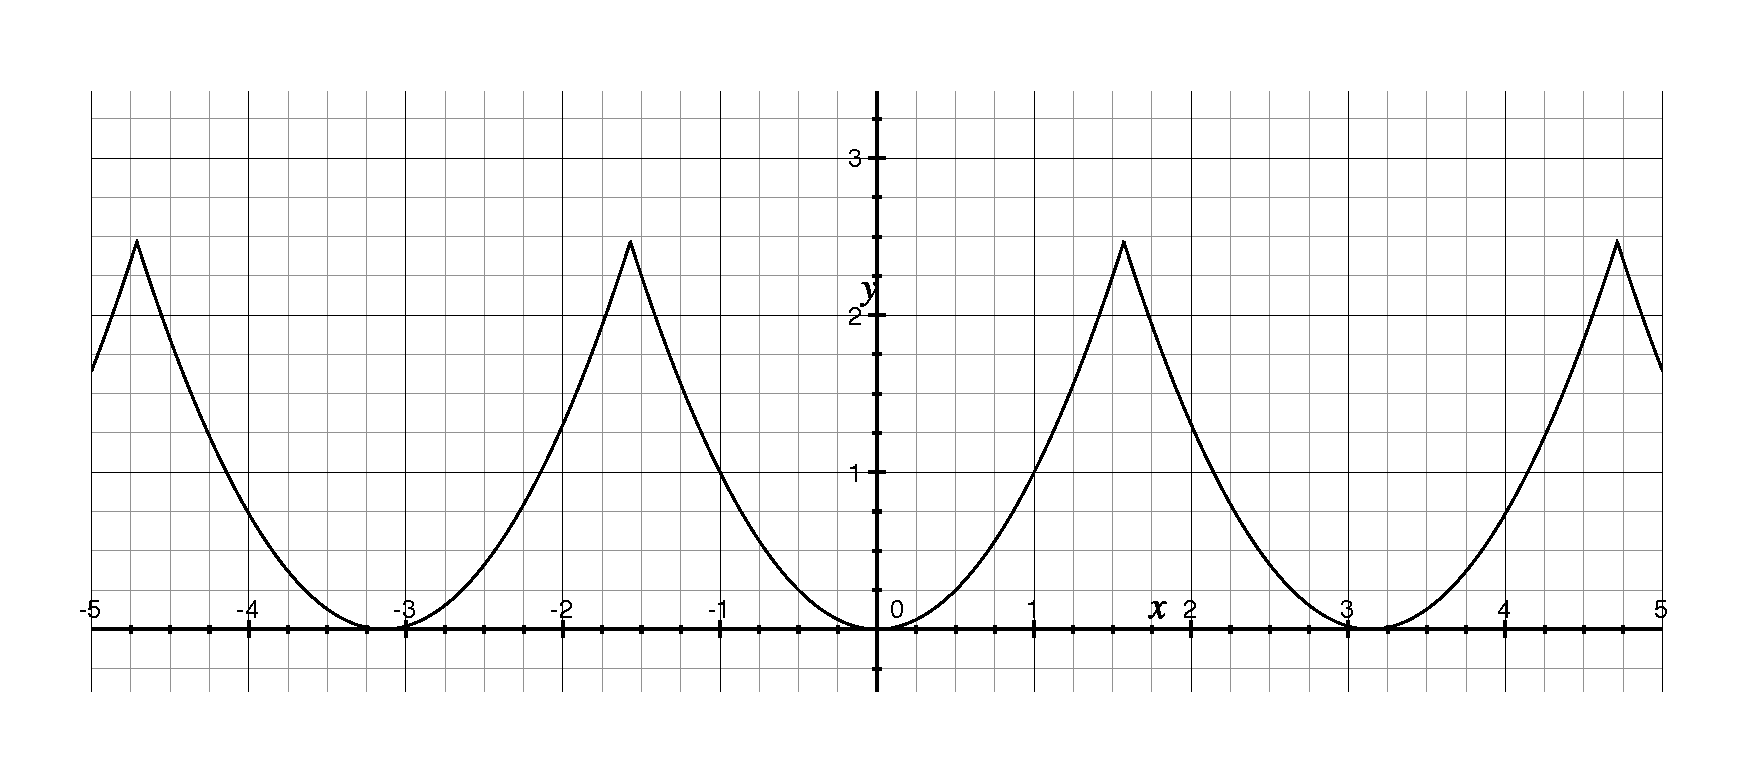
\includegraphics[scale=0.2]{grafy/graf1.eps}
\end{center}
\end{figure}
v bodě $x = \pi$ konverguje k $\pi^2$

\item $f(x) = x^2$ pro $x \in [0,2 \pi)$
\begin{figure}[!h]
\begin{center}
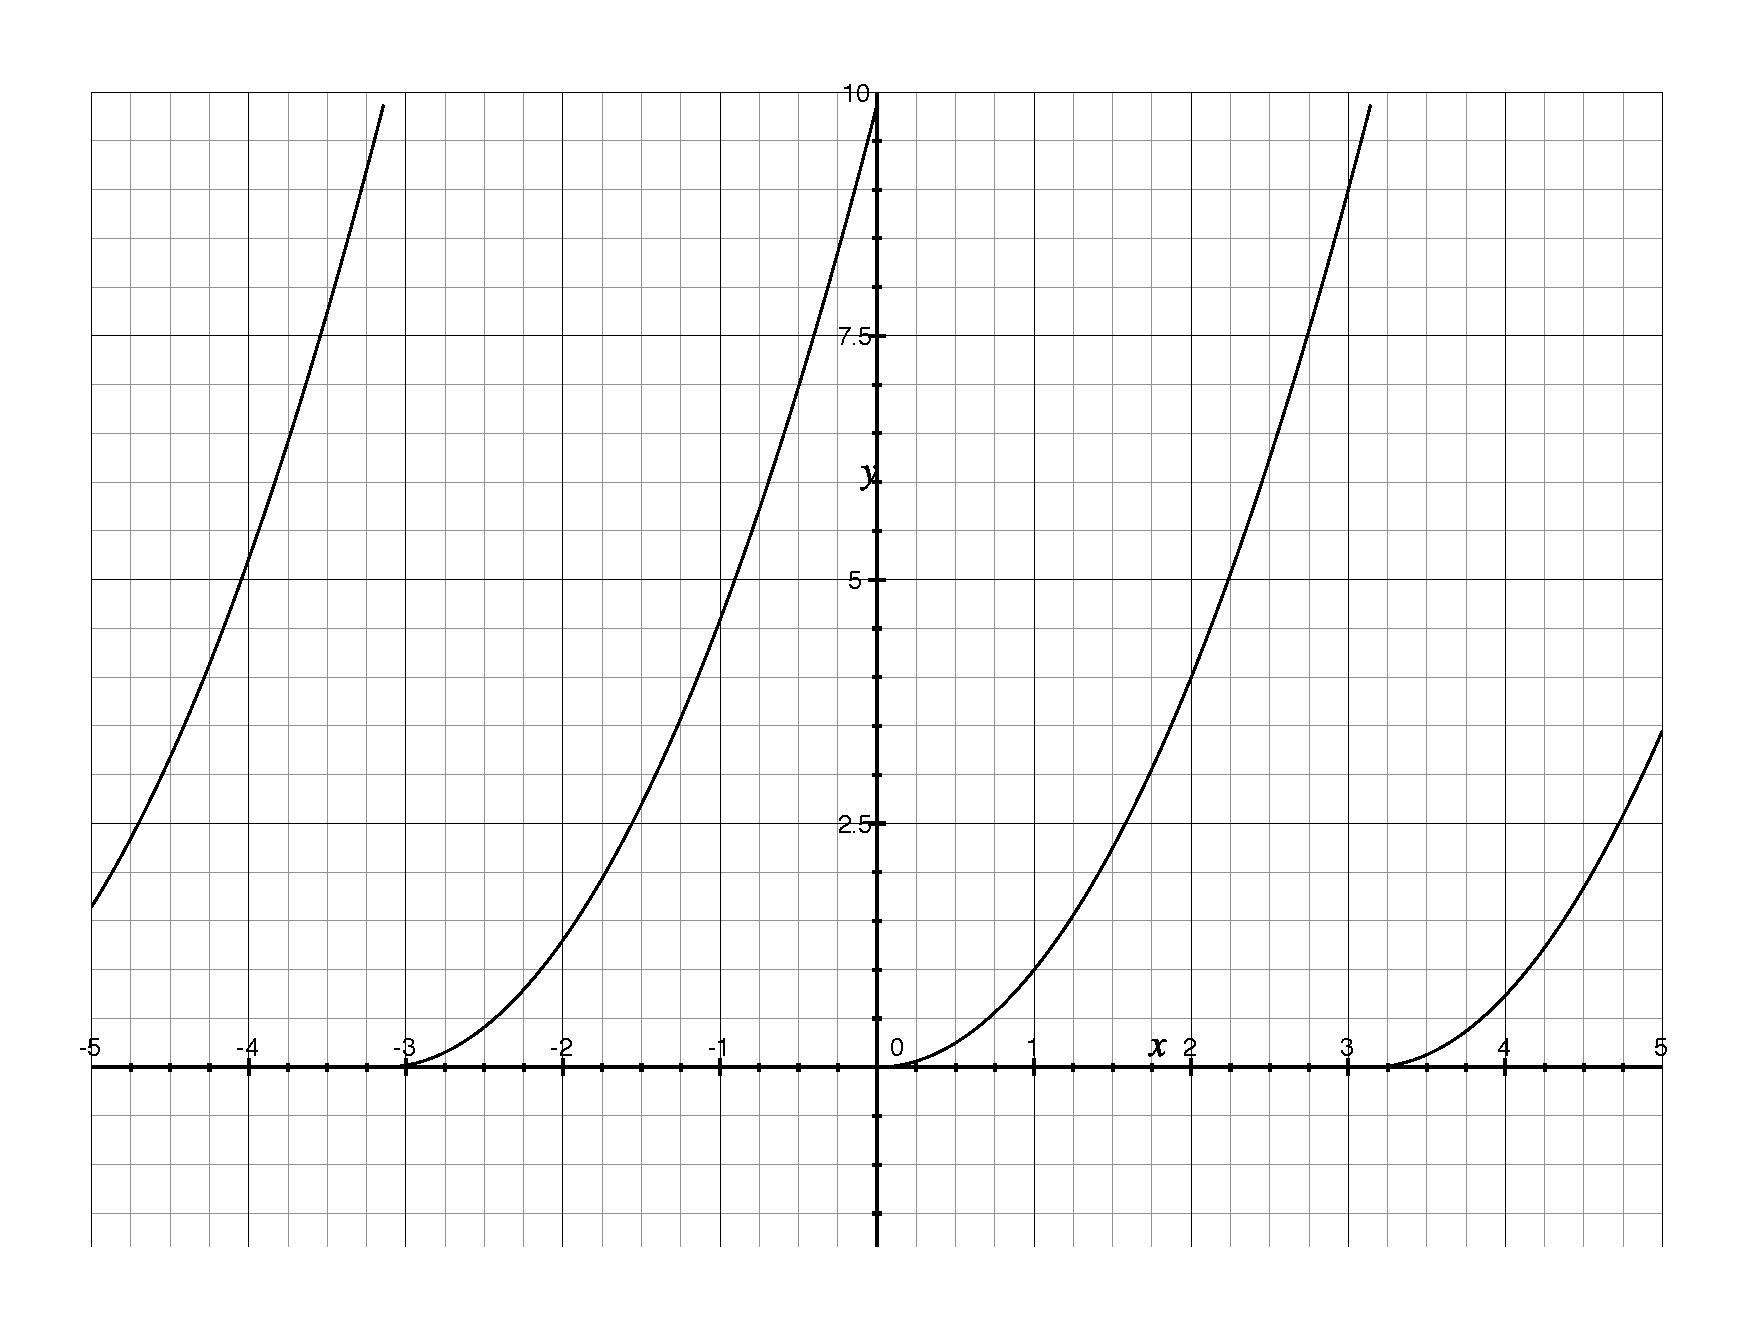
\includegraphics[scale=0.2]{grafy/graf2.eps}
\end{center}
\end{figure}
v bodě $x = 2\pi$ konverguje k $2\pi^2$

\end{itemize}
\end{priklad}


\begin{proof}
Chceme $F_f(x) = \frac{f(x+) + f(x-)}{2}$, tedy $s_n(x) \overset{n \rightarrow \infty}{\rightarrow}$

\begin{eqnarray*}
s_n(x) - \frac{f(x+)+f(x-)}{2} & = & \frac{1}{\pi} \int_0^\pi \left( f(x+y) + f(x-y) \right) D_n(y) dy - \frac{f(x+) + f(x-)}{2} \frac{2}{\pi} \int_0^\pi D_n(y)dy \\
& \overset{V5, VL4 (ii)}{=} & \frac{1}{\pi} \int_0^\pi \left( f(x+y) - f(x+) + f(x-y) - f(x-) \right) D_n(y) dy \\
& \overset{VL4(iii)}{=} & \frac{1}{\pi} \int_{0}^\pi \underbrace{\left( \frac{f(x+y) - f(x+) + f(x-y) - f(x-)}{2 \sin \left( \frac{y}{2} \right)} \right)}_{\textrm{pokud $\in R([0,\pi])$, pak VT\ref{Riemann-Lebesqueovo lemma} dokončí důkaz}} \sin \left( n + \frac{1}{2} \right)y dy 
\end{eqnarray*}

Chceme $F(y) = \frac{f(x+y) - f(x+) + f(x-y) - f(x-)}{2 \sin \left( \frac{y}{2} \right)} \in R([0,\pi])$. 

Existuje
$$\lim_{y \rightarrow 0} F(y) = \lim_{x \rightarrow 0} \frac{y}{2 \sin \left( \frac{x}{2} \right)} \lim_{y \rightarrow 0} \left( \frac{f(x+y)-f(x+)}{y} + \frac{f(x-y)-f(x-)}{y} \right) = A \in \mathbb{R}$$

\begin{tvrzeni}
$h \in R([a,b])$ spojitá na $[a,b]$, $0 < \delta \leq g \leq D$. Pak $\frac{h}{g} \in R([a,b])$.
\end{tvrzeni}

Nechť $\varepsilon > 0 \ \exists \delta > 0 \ \forall y \in [0, \delta] \textrm{ : } |F(y)-A| < \varepsilon$

Nyní $\delta$ je pevné a tedz dle tvrzení $F(y) \in R([\delta, \pi])$, $g(y) = 2 \sin \frac{y}{2}$.

Tedy $\exists \overline{D}$ dělení $[\delta, \pi]$ že $S(F,\overline{D}) - s(f,\overline{D}) < \varepsilon$.

Nechť $D$ je dělení $[0,\pi]$ mající interval k $\overline{D}$ a interval k $[0, \delta]$. Pak 
$$S(F, D)-s(f,D) = \left( \max_{x \in [0, \delta]} F(x) - \min_{x \in [0, \delta]} F(x) \right) \delta + S(F, \overline{D}) - s(F, \overline{D}) \leq 2 \varepsilon \delta + \varepsilon \leq \varepsilon (2 \pi + 1)$$
\end{proof}

\begin{vetabd}[Jordan-Dirichletovo kriterium]
Nechť $f \in \mathcal{P}_{2\pi}$ je po částech monotónní. Tedy nechť existuje konečně mnoho bodů $0=a_1 < a_2 < \ldots < a_m = 2 \pi$ tak, že $f$ je monotónní na $(a_i, a_{i+1})$ pro $i \in \{1, \ldots, m-1 \}$. Potom Fourierova řada funkce $f$ konverguje v bodě $x$ k hodnotě $\frac{f(x+) + f(x-)}{2}$ pro všechna $x \in \mathbb{R}$.
\end{vetabd}

\pagebreak
\setcounter{vety}{0}
\section{Základy komplexní analýzy}

Připomenutí vlastností $\mathbb{C}$ a operací $+$ a $\times$ na $\mathbb{C}$. Limita posloupnosti $z_n = a_n + i b_n \in \mathbb{C}$ je definována jako $\lim_{n \rightarrow \infty} a_n + i \lim_{n \rightarrow \infty} b_n$, pokud obě limity reálných čísel existují.

\subsection{Holomorfní funkce a křivkový integrál}

\begin{definice}
Nechť $f$ je funkce definovaná na okolí bodu $z_0 \in \mathbb{C}$ a zobrazující do $\mathbb{C}$. Komplexní derivací $f$ v $z_0$ nazýváme komplexní číslo
$$f^\prime (z_0) = \lim_{z \rightarrow z_0} \frac{f(z) - f(z_0)}{z - z_0}$$
pokud tato limita existuje.
\end{definice}

\begin{definice}
Nechť $G \subset \mathbb{C}$ je otevřená. Funkce $f : G \rightarrow C$ se nazývá \emph{holomorfní}, má-li ve všech bodech $G$ komplexní derivaci.
\end{definice}

\begin{poznamka}
Jsou-li $f$ a $g$ holomorfní na $G$, pak jsou $f+g$ i $f g$ holomorfní na $G$ a $f/g$ je holomorfní na $G \cap \{g \neq 0\}$.
\end{poznamka}

\begin{definice}
Zobrazení $\varphi : [a,b] \rightarrow \mathbb{C}$ je křivka a $f : \langle \varphi \rangle \rightarrow \mathbb{R}$ je spojité zobrazení. Definujeme křivkový integrál
$$\int_{\langle \varphi \rangle} f(z) dz = \int_\alpha^\beta f( \varphi (t)) \varphi^\prime(t) dt$$
existuje-li integrál na pravé straně. Tento integrál můžeme značit i $\int_\varphi f(z) dz$.
\end{definice}

\begin{vetat}[Cauchyho věta pro trojúhélník]
Nechť $f$ je holomorfní na otevřené množině $G \subset \mathbb{C}$ a $\Delta \subset G$ je trojúhelník. Pak $\int_{\delta \Delta} f(z) dz = 0$.
\end{vetat}

\begin{proof}
Sporem : nechť $\int_{\partial \triangle} f = M > 0$. Rozdělíme na čtyři trojúhelníky.

% TODO doplnit obrázek

Sečteme $\int$ přes hranice $\triangle_1$, $\triangle_2$, $\triangle_3 + \triangle_4$ v opačném směru.

Platí 
$$\int_{\partial \triangle_4} f = \int_{\partial \triangle_1} f + \int_{\partial \triangle_2} f + \int_{\partial \triangle_3} f + \int_{\partial \triangle_4} f$$

Tady $\exists \triangle_i \textrm{ : } \left| \int_{\partial \triangle_i} f \right| \geq \frac{M}{4}$. Tento trojúhelník opět rozdělíme na čtyři kusy. Dostaneme posloupnost trpjúhelníků $\triangle^K$ tak, že 
$$\left| \int_{\partial \triangle^K} f \right| \geq \frac{M}{4^K}$$
a
$$(\textrm{obvod $\triangle^K$}) = \frac{\textrm{obvod $\triangle$}}{2^K}$$

$\triangle^K$ uzavřené, zanořené do sebe $\Rightarrow$ 
$$\exists x_0 \in \bigcap_{K=1}^{\infty} \triangle^K$$
(důkaz přes konvergentní Cauchyovskou posloupnost)

Funkce $f$ je diferencovatelná v $x_0$, tady $f(z) = f(z_0) + f^\prime(z_0)(z-z_0) + \varepsilon (z-z_0)(z-z_0)$
$$\lim_{z \to z_0} \varepsilon (z-z_0) = 0$$

$$\left| \int_{\partial \triangle^K} f(z) dz \right| = \left| \int_{\partial \triangle^K} \underbrace{f(z_0) + f^\prime (z_0)(z-z_0)}_\circledast + \varepsilon (z-z_0) (z-z_0) dz \right|$$

$\circledast$ : má primitivní funkci $f(z)z + f^\prime(z_0) \frac{(z-z_0)^2}{2}$ a $\partial \triangle_K$ je uzavřená křivka, tedy 
$$\int_{\partial \triangle^K} \left[ f(z_0) + f^\prime (z_0) (z-z_0) \right] = 0$$

$$\frac{M}{4^K} \leq \left| \int_{\partial \triangle^K} f(z) dz \right| = \left| \int_{\partial \triangle^K} \varepsilon (z-z_0) (z-z_0) dz \right| \leq \textrm{délka } \partial \triangle_K \sup_{z \in \partial \triangle_K} \left| \varepsilon (z-z_0) \right| \sup_{z \in \partial \triangle_K} \left| z-z_0 \right| $$
$$ \leq \frac{c}{2^K} \varepsilon_K \frac{c}{2^K} \Rightarrow M \leq c^2 \varepsilon_K \overset{k \to \infty}{\rightarrow} 0 \Rightarrow M \leq 0$$

a to je spor.
\end{proof}

\begin{vetabd}[Cauchy]
Nechť $f$ je holomorfní na otevřené množině $G \subset \mathbb{C}$. Nechť $\langle \varphi \rangle \subset G$ je uzavřená křivka taková, že vnitřek $\langle \varphi \rangle \subset G$ (tedy případné "díry" uvnitř G nejsou uvnitř $\langle \varphi \rangle$). Pak $\int_\varphi f(z)dz=0$.
\end{vetabd}

\begin{vetal}[Cauchyův vzorec]
\label{Cauchyův vzorec}
Nechť $f$ je holomorfní na kruhu $B(z_0, R)$ a $0<r<R$. Pro křivku $\varphi(t) = z_0 + r e^{it}$, $t \in [0,2\pi]$, platí

\begin{equation}
\frac{1}{2 \pi i} \int_\varphi \frac{f(z)}{z-s}  = \left\{ \begin{array}{ll}
 f(z) & \textrm{pro $|s-z_0| < r$} \nonumber\\
 0 & \textrm{pro $| s-z_0 | > r$}
  \end{array} \right.
\end{equation}
\end{vetal}

\begin{proof}
\begin{enumerate}
\item $|s-z_0| > r$

pak $\frac{f(z)}{z-s}$ je holomorfní na $B(z_0, r + \varepsilon)$ dle Cauchyho věty

$$\int_\varphi \frac{f(z)}{z-s} dz = 0$$

\item $|s-z_0| < r$

Definujme funkce 
\begin{equation}
F(z)  = \left\{ \begin{array}{ll}
 \frac{f(z)-f(s)}{z-s} & \textrm{pro $z \neq s$} \nonumber\\
 f^\prime(s) & \textrm{pro $z=s$}
  \end{array} \right.
\end{equation}

Pak $F(z)$ je holomorfní na $B(z_0, R) \backslash \{ s \}$ a v $s$ spojitá. Dle Poznámky

$$\int_\varphi F(z) dz = 0 = \int_\varphi \frac{f(z)}{z-s} dz - \int_\varphi \frac{f(s)}{z-s} dz$$
\end{enumerate}
\end{proof}


\begin{vetat}[Liouville]
\label{Liouville}
Nechť $f$ je holomorfní a omezená na $\mathbb{C}$. Pak $f$ je konstantní.
\end{vetat}

\begin{proof}
Nechť $\varphi (t) = R e^{it}$. Podle Věty \ref{Cauchyův vzorec} (Cauchyův vzorec) máme
$$f(s) = \frac{1}{2 \pi i} \int_\varphi \frac{f(z)}{z-s}dz \qquad \circledcirc$$

$(\int \quad)^\prime = (\int (\quad)^\prime)$. Poznámka p. doc. Hencla: "Vy to udělat nemůžete, já ano, protože jsem absolvoval přednášku z teorie míry a integrálu."

Tedy $|f^\prime (s)| \leq \frac{1}{2 \pi} 2 \pi R \sup_{z \in \mathbb{C}} |f(z)| \frac{1}{| R - |s| |^2} \overset{R \to \infty}{\to} 0$

$$f^\prime (s) = 0 \ \forall s \in \mathbb{C} \Rightarrow \textrm{$f$ je konstantní}$$

Nyní stačí ukázat, že mužeme udělat $(\int \quad)^\prime = (\int (\quad)^\prime)$.

Připomeň: $F_n \con F$, pak $\int F_n \to \int F$ (pro $\mathbb{R} \to \mathbb{R}$, také pro $\mathbb{R} \to \mathbb{C}$)

Lze použít i pro $\int_\varphi F = \int_\alpha^\beta F(\varphi(t)) \varphi^\prime (t) dt \Rightarrow \lim_{n \to \infty} \int F_n = \int \lim_{n \to \infty} F_n$

$$f^\prime (s) = \lim_{h \to 0} \frac{f(s+h)-f(s)}{h} \overset{\circledcirc}{=} \lim_{h \to 0} \frac{1}{h} \left( \int_\varphi \frac{f(z)}{z-(s+h)} dz - \int_\varphi \frac{f(z)}{z-s} dz \right) = \lim_{h \to 0} \int_\varphi f(z) \frac{1}{h} \left( \frac{1}{z-(s+h)} - \frac{1}{z-s} \right) dz = \lim_{h \to 0} \int_\varphi f(z) \frac{1}{(z-(s+h))(z-s)} dz$$

Pohle Heineho stačí 
$$\lim_{n \to \infty} \int_\varphi \underbrace{f(z) \frac{1}{(z-(s+h_n))(z-s)}}_{F_n(z)} dz$$
pro $h_n \to 0$

!!! ZDE CHYBÍ KOUSEK !!!, potom $\lim \int = \int \lim_{n \to \infty} = \int_\varphi f(z) \frac{1}{(z-s)^2} dz$

$F_n(z) \con F(z)$

$$|F_n(z)-F(z)| = |f(z)| \left| \frac{1}{(z-(s+h_n))(z-s)} - \frac{1}{(z-s)^2} \right| \leq \sup_{z \in \langle \varphi \rangle} |f(z)| \max \frac{1}{|z-s|} \frac{|h_n|}{|\underbrace{(z-(s+h_n))}_{\leq \frac{1}{2} (z-s)}(z-s)|}$$
\end{proof}


\begin{vetal}[Základní věta algebry]
Každý nekonstantní polynom (s komplexními koeficienty) má v $\mathbb{C}$ alespoň jeden kořen.
\end{vetal}

\begin{proof}
Sporem. Nechť $\forall z \in \mathbb{C} \textrm{ : } P(z) \neq 0$. Pak $\frac{1}{P(z)}$ he holomorfní funkce na $\mathbb{C}$.

$$P(z) = a_n z^n + a_{n-1} z^{n-1} + \ldots + a_0 = a_n z^n \left( 1 + \frac{a_{n-1}}{a_n} \frac{1}{z} + \ldots + \frac{a_0}{a_n} \frac{1}{z^n} \right)$$

$\exists R > 0 \ \forall |Z| > R \textrm{ : }$

$$\left( 1 + \frac{a_{n-1}}{a_n} \frac{1}{z} + \ldots + \frac{a_0}{a_n} \frac{1}{z^n} \right) > \frac{1}{2} \geq 1 - \frac{|a_{n-1}|}{|a_n|} \frac{1}{R} - \frac{|a_{n-2}|}{|a_n|} \frac{1}{R^2} - \ldots - \frac{|a_0|}{|a_n|} \frac{1}{R^n}$$

Tedy 
$$\left| \frac{1}{P(z)} \right| \leq \frac{1}{|a_n z^n| (\ldots)} \leq \frac{2}{|a_n| |z^n|}$$

Tedy $\frac{1}{P(z)}$ je omezená holomorfní funkce, tedy dle Věty \ref{Liouville} je $\frac{1}{P(z)}$ konstantní a to je spor.
\end{proof}


\subsection{Rozvoj do Taylorovy a Laurentovy řady}

\begin{definice}
Nehcť $z_0 \in \mathbb{R}$ a $a_n \in \mathbb{C}$ pro $n \in \mathbb{N}_0$. Řadu funkcí $\sum_{n=0}^{\infty} a_n (z-z_0)^n$ pro $z \in \mathbb{C}$ nazýváme mocninnou řadou s koeficienty $a_n$ o středu $z_0$.
\end{definice}

\begin{vetat}[o rozvoji do Taylorovy řady]
Nechť $f$ je holomorfní na kruhu $B(z_0, R)$. Pak existuje právě jedna mocninná řada s poloměrem konvergence alespoň $R$, že na $B(z_0, R)$ platí
$$f(z) = \sum_{n=0}^\infty a_n (z-z_0)^n$$
Navíc platí $a_n = \frac{f^{(n)}(z_0)}{n!}$ pro všechna $n \in \mathbb{N}_0$.
\end{vetat}

Jako u reálných mocninných řad lze na kruhu konvergence prohazovat $\sum$ a derivaci a důkaz je podobný.

\begin{dusledek}
Je-li $f$ holomorfní na $G$, pak na $G$ existují derivace všech řádů $f^{(k)}$ pro $k \in \mathbb{N}$.
\end{dusledek}

\begin{definice}
Množina $G \subset \mathbb{C}$ se nazývá \emph{oblast}, pokud je otevřená a souvislá. Tedy pokud platí
$$\forall A, B \in G \textrm{ otevrene v } G, G=A \cup B, A \cap B = \emptyset \Rightarrow A = \emptyset \textrm{ nebo } B = \emptyset$$
\end{definice}

\begin{vetal}[o jednoznačnosti holomorfní funkce]
Nechť $G \subset \mathbb{C}$ je oblast a $f, g$ jsou holomorfní na $G$. Předpokládejme, že množina
$$M = \left\{ z \in G : f(z)=g(z) \right\} $$
má hromadný bod v $G$, neboli existují $z_n \in M$ a $z_0 \in G$ takové, že $z_n \stackrel{n \rightarrow \infty}{\rightarrow} z_0$. Pak $f=g$ na $G$.
\end{vetal}

\begin{dusledek}
$\sin^2 (z) + \cos^2 (z) = 1$ platí $\forall z \in \mathbb{C}$, neboť platí na $\mathbb{R}$ - reálná osa $\to$ úsečka
\end{dusledek}


\begin{definice}
Řekneme, že funkce $f$ má v bodě $z_0$ pól násobnosti nejvýše $k \in \mathbb{N}$, je-li funkce 
\begin{equation}
F(z) = \left\{ \begin{array}{ll}
 (z-z_0)^{k+1}f(z) & \textrm{pro $z \neq z_0$} \nonumber\\
 0 & \textrm{pro $z=z_0$}
  \end{array} \right.
\end{equation}

holomorfní na nějakém okolí bodu $z_0$. Řekneme, že má pól násobnosti $k$, je-li $k \in \mathbb{N}$ nejmenší s touto vlastností.
\end{definice}

Například funkce $f(z) = 1 / z^k$ má v bodě 0 pól násobnosti k.

\begin{definice}
Nechť $M \subset G \subset \mathbb{C}$ je konečná množina. Řekneme, že funkce $f : G \backslash M \rightarrow \mathbb{C}$ je \emph{meromorfní} v $G$, pokud je $f$ holomorfní na $G \backslash M$ a v bodech $M$ má $f$ póly (konečné násobnosti).
\end{definice}

\begin{vetat}[o rozovji do Laurentovy řady]
Nehcť $f$ je holomorfní na mezikruží $B(z_0, R) \backslash \overline{B(z_0, r)}$, $0 < r < R$. Pak existují jednoznačně určená čísla $a_k \in \mathbb{C}$, $k \in \mathbb{Z}$, že platí 
$$f(z) = \sum_{k= - \infty}^\infty a_k (z-z_0)^k \textrm{ pro všechna } z \in B(z_0, R) \backslash \overline{B(z_0, r)}$$
\end{vetat}

\subsection{Reziduová věta a její aplikace}

\begin{definice}
Nechť $\sum_{k =- \infty}^\infty a_k ( z-z_0)^k$ je Laurentova řada funkce $f$. \emph{Rezuduum} funkce $f$ v bodě $z_0$ nazveme koeficient $a_{(-1)}$ a značíme ho $res_{z_0} f$.
\end{definice}

\begin{definice}
\emph{Index bodu $z_0$} vzhledem v uzavřené křivce $\varphi$ je definován jako
$$\mathrm{ind}_\varphi z_0 = \frac{1}{2 \pi i} \int_\varphi \frac{1}{z-z_0}dz$$
\end{definice}

Index bodu udává, kolikrát oběhne křivka $\varphi$ okolo bodu $z_0$, pokud uvažujeme násobnost a obíhání v opačném směru bereme s opačným znaménkem.

\begin{vetat}[Reziduová věta]
Nechť $G \subset \mathbb{C}$ je oblast, $f$ je meromorfní funkce na $G$, $\varphi$ je křivka a póly $f$ neleží na $\langle \varphi \rangle (\subset G)$. Pak platí
$$\int_\varphi f(z) dz = 2 \pi i \sum_{\{z: z \textrm{ je pól } f\}} \mathrm{res}_z (f) \mathrm{ind}_z (f)$$
\end{vetat}

\begin{proof}
Označme $P = \left\{ z \in G \textrm{ : } f(z)=+\infty \textrm{ resp. $f$ má pól v $z$} \right\}$. 
Pro $z_0 \in G$ označme 
$$H_{z_0} = \sum_{k = -kz}^{-1} a_k (z-z_0)^k$$ 
část rozvoje $f$ do Laurentovy řady.
Pak $$F(z) = f(z) - \sum_{z_0 \in P} H_{z_0}(z)$$ je $F$ holomorfní na $G$.
Podle Cauchyovy věty $\int_\varphi F(z) dz = 0$. Tedy
\begin{eqnarray*}
\int_\varphi F(z) dz & = & \int_\varphi \sum_{z_0 \in P} H_{z_0}(z) dz \\
& = & \sum_{z_0 \in P} \sum_{k=-kz}^{-1} \int_\varphi a_k (z-z_0)^k dz \\
& = & \sum_{z_0 \in P} res_{z_0} f \int_\varphi \frac{1}{z-z_0} dz \\
& = & 2 \pi i \sum_{z_0 \in P} res_{z_0} f ind_\varphi z_0 
\end{eqnarray*}
\end{proof}

\subsubsection*{Pravidla pro výpočet rezidua}

\begin{enumerate}
\item Je-li $h$ holomorfní na okolí $a$ a $g$ má v $a$ jednoduchý pól, pak
$$res_a(hg) = h(a) res_a (g)$$
\item Jsou-li $h$, $g$ holomorfní na okolí $a$ a $g$ má v $a$ jednoduchý kořen, pak 
$$res_a \left( \frac{h}{g} \right) = \frac{h(a)}{g \prime (a)}$$
\item Má-li $f$ v $a$ pól násobnosti $n$, pak lze reziduum spočítat za pomoci derivování řádu $(n-1)$ jako
$$res_a(f) = \lim_{z \rightarrow a} \frac{1}{(n-1)!} \left[ (z-a)^n f(z) \right]^{(n-1)}$$
\end{enumerate}

\subsubsection*{Výpočet integrálů za pomoci reziduové věty:}

Nechť $Q$ je racionální funkce.

\begin{enumerate}
\item $\int_0^{2\pi} Q(\cos(t), \sin(t))dt$

substituce $e^{it} = z$, $\cos(t) = \frac{z + \frac{1}{z}}{2}$, $\sin(t) = \frac{z-\frac{1}{z}}{2i}$, $\frac{dz}{dt} = e^{it}i$

\item $\int_{-\infty}^\infty R(x) dx$
$$\left| \int_{\varphi_1} R(z) dz \right| \leq \pi R \frac{c}{R^2} \overset{R \to \infty}{\to} 0$$

$R = \frac{P}{Q}$, stupeň $Q$ $\geq$ stupeň $P + 2$, $\forall t \in \mathbb{R} \textrm{ : } R(t) \neq \infty$
$$\int_{-\infty}^\infty R(t) dt = 2 \pi i \sum_{ \{ z_0 \in \mathbb{C} \textrm{ : } R(z_0) = \infty \} } \textrm{res}_{z_0} R(z)$$

\item $\int_{-\infty}^{\infty} Q(x) \sin(x) dx$
\item $\int_{-\infty}^{\infty} Q(x) \cos(x) dx$
\item $\int_0^{\infty} Q(x) x^{p-1} dx$
\end{enumerate}

\pagebreak
\setcounter{vety}{0}
\section{Metrické prostory II}

\begin{definice}
\emph{Metrickým prostorem} budeme rozumět dvojici $(P, \varrho)$, kde $P$ je množina bodů a $\varrho : P \times P \rightarrow \mathbb{R}$ splňuje 

\begin{enumerate}
\item $\forall x,y \in P \textrm{ : } \varrho(x,y) = 0 \Leftrightarrow x = y$
\item $\forall x,y \in P \textrm{ : } \varrho(x,y) = \varrho(y,x) \qquad \textrm{(symetrie)}$
\item $\forall x,y,z \in P \textrm{ : } \varrho(x,z) \leq \varrho(x,y) + \varrho(x,z) \qquad \textrm{(trojúhelníková nerovnost)}$
\end{enumerate}
Funkce $\varrho$ nazýváme \emph{metrika}.
\end{definice}

\begin{definice}
Nechť $(P, \varrho)$ je metrický prostor a $\{ x_n \}_{n=1}^\infty$ je posloupnost prvků $P$ a $x \in P$. Řekneme, že $\{ x_n \}_{n=1}^{\infty}$ \emph{konverguje k $x$ (v $(P, \varrho)$)}, pokud $\lim_{n \rightarrow \infty} \varrho(x_n, x) = 0$. Značíme $\lim_{n \rightarrow \infty} x_n = x$, nebo $x_n \overset{\varrho}{\rightarrow} x$.
\end{definice}

\begin{definice}
Nechť $(P, \varrho)$ je metrický prostor v $K \subset P$. Řekneme, že $K$ je \emph{kompaktní}, jestliže z každé posloupnosti prvků $K$ lze vybrat konvergentní podposloupnost s limitou v $K$.
\end{definice}

\begin{vetabd}[charakterizace kompaktních množin $\mathbb{R}^n$]
Množina $K \subset \mathbb{R}^n$ je kompaktní, přávě když je omezená a uzavřená.
\end{vetabd}

\begin{vetal}[nabývání extrémů na kompaktu]
Nechť $(P, \varrho)$ je metrický prostor a $K \subset P$ je kompaktní. Nechť $f \textrm{ : } K \rightarrow \mathbb{R}$ je spojitá. Pak $f$ nabývá na $K$ svého maxima i minima. Speciálně je tedy $f$ na $K$ omezená.
\end{vetal}

\begin{proof}
Z definice suprema :
$$\exists x_n \in K \textrm { : } \lim_{n \to \infty} f(x_n) = \sup_{x \in K} f(x)$$
$K$ je kompaktní interval, tedy $\exists x_{n_k} \to x_n \in K$. Z Heineho věty (Heine: $y_n \to y$, $f$ spojitá $\Rightarrow$ $f(x_n) \to f(y)$) a spojitosti $f$ dostáváme 
$$\lim_{k \to \infty} \underbrace{f(x_{n_k})}_{\sup_{x \in K} f(x)} = f(x_0)$$
Tedy v $x_0$ nabývá $f$ maxima. Pro minimum analogicky
\end{proof}



\addtocounter{subsection}{1}
\subsection{Úplné metrické prostory}

\begin{definice}
Nechť $(P, \varrho)$ je metrický prostor a nechť $x_n \in P, n \in \mathbb{N}$, je posloupnost bodů z $P$. Posloupnost $\{ x_n \}_{n \in \mathbb{N}}$ nazveme \emph{cauchyovskou}, pokud
$$\forall \varepsilon > 0 \ \exists n_0 \in \mathbb{N} \ \forall m,n \geq n_0 \textrm{ : } \varrho(x_n, x_m) < \varepsilon$$
Posloupnost $\{ x_n \}_{n \in \mathbb{N}}$ nezveme \emph{konvergentní}, pokud existuje $x \in P$ tak, že
$$\lim_{n \rightarrow \infty} \varrho (x_n, x) = 0$$
Řekneme, že $(P, \varrho)$ je \emph{úplný}, pokud je každá cauchzovská poslouopnost konvergentní.
\end{definice}

\begin{vetal}[úplnost $\mathbb{R}^n$]
Metrický prostor $(\mathbb{R}, |.|)$ je úplný.
\end{vetal}

\begin{priklad}
\begin{enumerate}
\item Metrický prostor $(Q, |.|)$ není úplný.
\item Metrický prostor všech spojitých funkcí $C([0, 1])$ s metrikou
$$\varrho_1(f,g) = (R) \int_0^1 |f(x) - g(x)| dx$$
není úplný.
\item Metrický prostor všech Lebesqueovsky integrovatelných funkcí $L([0,1])$ s metrikou
$$\varrho(f,g) = (L) \int_0^1 |f(x)-g(x)|dx$$
je úplný
\end{enumerate}
\end{priklad}

\begin{vetat}[úplnost spojitých funkcí]
Metrický prostor spojitých funkcí $(C([0,1]), \varrho)$ se supremovou metrikou
$$\varrho(f,g) = \sup_{x \in [0,1]} |f(x) - g(x)|$$
je úplný
\end{vetat}

\begin{vetat}[Banachova věta o kontrakci]
\label{Banachova věta o kontrakci}
Nechť $(P, \varrho)$ je úplný metrický prostor a $K < 1$. Nechť $T \textrm{ : } P \rightarrow P$ je zobrazení takové, že 
$$\varrho(Tx, Ty) \leq K \varrho(x,y) \quad \forall x,y \in P$$
Pak existuje právě jeden bod $x_0 \in P$ tak, že $T(x_0)=x_0$
\end{vetat}

\begin{proof}
\textbf{jednoznačnost: } Nechť $T(x_0) = x_0$ a $T(\tilde{x}_0) = \tilde{x}_0$, $x_0 \neq \tilde{x}_0$. Pak 
$$K \varrho (x_0, \tilde{x}_0) \geq \varrho (T(x_0),T(\tilde{x}_0)) = \varrho (x_0, \tilde{x}_0) \Rightarrow K \geq 1$$
a to je spor.

\textbf{existence: } Zvolme $x_1 \in P$ libovolně a položme $x_{k+1} = T(x_k)$. Tvrdíme, že je cauchyovská.
$$\varrho( x_{k+1}, x_k ) = \varrho (T(x_k), T(x_{k-1})) \leq K \varrho (x_k,x_{k-1}) \leq K^2 \varrho (x_{k-1},x_{k-2}) \leq \ldots \leq K^{k-1} \varrho (x_2, x_1)$$

Nechť $m,n \geq n_0$ a navíc $m > n$
$$\varrho (x_m, x_n) \leq \varrho (x_m, x_{m-1}) + \varrho (x_{m-1}, x_{m-2}) + \ldots + \varrho (x_{n+1}, x_n) $$
$$\leq K^{m-2} \varrho (x_2, x_1) + \ldots + K^{n-1} \varrho (x_2, x_1) \leq K^{n-1} \varrho (x_2, x_1) \frac{1}{1-K} \overset{x \to \infty}{\to} 0$$

Z toho dostaneme cauchyho vlastnost $x_2$. Z úplnosti $P$ $\exists x_0 \textrm{ : } x_n \overset{P}{\to} x_0$. Tvrdím $T(x_0)=x_0$
\begin{eqnarray*}
x_{n+1} & = & T(x_n) \\
\lim_{n \to \infty} \quad x_0 & = & T(x_0)
\end{eqnarray*}

$x_n \to x_0 \textrm{ : } \varrho (x_m, x_0) \to 0$, $\varrho (T(x_n), T(x_0)) \leq K \varrho (x_n, x_0) \to 0$
\end{proof}

\begin{poznamka}
Věta T\ref{Banachova věta o kontrakci} se používá například v \emph{fractal compression}. Touto metodou se však dosahuje horších výsledků než například konpresí \emph{JPEG} a proto se v praxi nepoužívá.
\end{poznamka}



\begin{vetat}[o zúplnění metrického prostoru]
Nechť $(Q, \varrho)$ je metrický prostor. Pak existuje úplný metrický prostor $(P, \sigma)$ tak, že $Q \subset P$ a 
$$\sigma(x,y) = \varrho(x,y) \quad \forall x,y \in Q$$
\end{vetat}

\begin{proof}
Položme $P = C(Q)$ s metrikou $\varrho (f,g) = \sup_{y \in Q} | f(x)-g(x) |$. 

\begin{poznamka} 
Důkaz je analogický a důkazu věty o úplnosti $C([0,1])$
\end{poznamka}

$x \in Q \textrm{ <$\cdots$> } f_x(y) = \varrho(x,y) \in C(Q)$. 

Pro $x \neq z$ a $f_x \neq f_z$ chceme $\sigma (x,z) = \varrho (f_x, f_z)$
$$\varrho (f_x, f_z) = \sup_{y \in Q} | \sigma (x,y) - \sigma (z,y) | \overset{\textrm{$\triangle$ nerovnost}}{\leq} \sigma (x,z) \Rightarrow \varrho (f_x, f_z) = \sigma(x,z)$$ 
\end{proof}


\begin{vetal}[úplnost a uzavřená podmnožina]
Nechť $(P, \varrho)$ je úplný metrický prostor a $F \subset P$ je uzavřená podmnožina. Pak je metrický prostor $(F, \varrho)$ úplný.
\end{vetal}

\begin{proof}
\textbf{Připomeň: } Charakterizace úplných množin: $F \subset F \textrm{uzavřená}$, $x_n \in F$ a $x_n \overset{P}{\to} x_0$ pak $x_0 \in F$. 

"Když je množina uzavřená, pak se z ní nelze vykonvergovat ven"

Chceme $(F, \varrho)$ je úplný. Nechť $x_n \in F$ je cauchyovská v $(P, \varrho)\Rightarrow x_n$ je cauchyovská v $(P, \varrho) \overset{\textrm{P je úplný}}{\Rightarrow} \exists x_0 \in P \textrm{ : } x_n \to x_0 \overset{\textrm{Připomeň}}{\Rightarrow} x_0 \in F$ tedy $(F, \varrho)$ je úplný.
\end{proof}


\pagebreak
\section*{Příklady}

\begin{multicols}{2}

Vyšetřete stejnoměrnou a lokálně stejnoměrnou konvergenci posloupnosti funkcí $f_n$ na intervalu $(0,1)$
$$f_n(x) = x^n - x^{3n}$$

\separator

Vyšetřete stejnoměrnou a lokálně stejnoměrnou konvergenci posloupnosti funkcí $f_n$ na intervalu $(-\infty,0)$
$$f_n(x) = e^{nx}$$

\separator

Vyšetřete stejnoměrnou a lokálně stejnoměrnou konvergenci funkcí na $\mathbb{R}$
$$\sum_{n=1}^\infty \sin \left( \frac{1}{x^2 + n^2} \right)$$

\separator

Určete poloměr konvergence následující řady
$$\sum_{n=1}^\infty 2^n x^{4^n}$$

\separator

Sečtěte řadu
$$\sum_{n=1}^{\infty} \frac{3^{-n}}{n}$$

\separator 

Najděte Fourierovu řadu následující funkce.
$$f(x) = (\textrm{sgn} x) \sin x \quad \textrm{na intervalu} \ [-\pi, \pi)$$

\separator

Najděte Fourierovu řadu následující funkce a zjistěte k jakým hodnotám konverguje
$$f(x)=x \textrm{ pro } x \in [0,\pi) \textrm{ a } f(x)=0 \textrm{ pro } x \in [-\pi,0)$$

\separator

Spočtěte integrál podle definice křivkového integrálu
$$\int_{S^1} \sqrt{z} + \frac{1}{\sqrt{z}} dz$$
kde $S^1$ je jednotková kružnice probíhaná v kladném smzslu a volíme $\sqrt{1}=1$

\separator

Najděte residua následující funkce
$$f(z)=\frac{z^2}{(1+z^2)^2}$$

\separator

Spočtěte
$$\int_{-\infty}^\infty \frac{1}{(x^2 + 9)^3} dx$$

\separator

Vyšetřete bodovou a stejnoměrnou konvergenci následujících funkcí
\begin{enumerate}
\item $f_n(x) = \frac{x^n}{1+x^n}$ na $[0,1]$
\item $f_n(x) = x^n - x^{2n}$ na $(0,1)$
\item $f_n(x) = \sin \left( \frac{x}{n} \right)$ na $(-100,100)$
\item $f_n(x) = n \left( \sqrt{x + \frac{1}{n}} - \sqrt{x} \right)$ na $(0,\infty)$
\item $f_n(x) = \sqrt[n]{1+x^n}$ na $(0,\infty)$
\item $f_n(x) = n \left( x^\frac{1}{n} - 1 \right)$ na $(1,100)$ a $(1,\infty)$
\end{enumerate}

\separator

Zjistěte, zda $f_n$ jdou stejnoměrně a lokálně stejnoměrně k nějaké $f$ na intervalu $J$
\begin{enumerate}
\item $f_n(x) = e^{n (x-1)}$, $J = (0,1)$
\item $f_n(x) = \sin (\pi x^n)$, $J = [0,1)$
\item $f_n(x) = \frac{nx}{1+n+x}$, $J = (0,\infty)$
\item $f_n(x) = n x e^{-nx^2}$, $J = \mathbb{R}$
\item $f_n(x) = \frac{\ln (nx)}{n}$, $J = (0,\infty)$
\item $f_n(x) = \left( 1 + \frac{x}{n} \right)^n$, $J = (0,\infty)$
\item $f_n(x) = x \arctan (nx)$, $J = \mathbb{R}$
\item $f_n(x) = x^{2n} - x^{3n}$, $J = (0,1)$
\item $f_n(x) = \sqrt{x^2 + \frac{1}{n^2}}$, $J = \mathbb{R}$
\item $f_n(x) = \sqrt{x} \sin \frac{x}{n}$, $J = \mathbb{R}$
\end{enumerate}

\separator

Zjistěte na kterách intervalech konverguje řada stejnoměrně resp. lokálně stejnoměrně.
\begin{enumerate}
\item $\sum_{n = 1}^\infty x^n$
\item $\sum_{n = 1}^\infty \frac{1}{n^2 x^2 + 1}$
\item $\sum_{n = 1}^\infty x^2 e^{-nx}$
\item $\sum_{n = 1}^\infty \ln \left( 1 + \frac{x^2}{n \ln^2 n } \right)$
\item $\sum_{n = 1}^\infty \arctan \left( \frac{2x}{x^2 + n^3} \right)$
\item $\sum_{n = 1}^\infty \frac{nx}{(1+x)(1+2x)\ldots(1+nx)}$ na $(0,\infty)$
\end{enumerate}

\separator

Zjistěte, zda $\sum_{n=0}^{\infty}$ je na $(a,b)$ diferencovatelná a zda konverguje lokálně stejnoměrně
\begin{enumerate}
\item $\sum_{n=1}^\infty \frac{1}{n^2 + x}$ na $(-1, \infty)$
\item $\sum_{n=1}^\infty (1-x^n) x^n$ na $[0,1]$
\item $\sum_{n=1}^\infty \frac{x^n}{n^s}$ na $[0, \infty)$ s parametrem $s \in \mathbb{R}$
\item $\sum_{n=1}^\infty \frac{\arctan \left( \frac{x}{n} \right)}{n}$ na $(-1, \infty)$
\item $\sum_{n=1}^\infty \frac{\sin \frac{x}{\sqrt{n}}}{x^2 + n}$ na $\mathbb{R}$
\item $\sum_{n=1}^\infty \sin \frac{1}{x^2 + n^2}$
\item $\sum_{n=1}^\infty 2^n \arctan ( 3^n x^n )$ na $[0,1]$
\end{enumerate}

\separator

Sečtěte řadu
\begin{enumerate}
\item $x - 4x^2 + 9x^3 - \ldots$
\item $\sum_{n=0}^\infty \frac{x^{4n+1}}{4n+1}$
\item $\sum_{n=0}^\infty \frac{n^2}{2^n}$
\end{enumerate}

\separator

Určete poloměr konvergence
\begin{enumerate}
\item $\sum_{n=1}^\infty \frac{z^n}{n^3}$
\item $\sum_{n=1}^\infty \frac{(n!)^2}{(2n)!} z^n$
\item $\sum_{n=1}^\infty \frac{z^{n!}}{n!}$
\item $\sum_{n=1}^\infty \left( na^n + \frac{b^n}{n^2} \right) z^n$ pro $0 < a < b$
\item $\sum_{n=1}^\infty \frac{n!}{a^{n^2}} z^n$ pro $a > n$
\end{enumerate}

\separator

Spočtěte $\int_C \frac{1}{\sqrt{z}} dz$, kde $C$ je jednotková kružnice probíhající v kladném smyslu

\separator

Spočtěte $\int_C z dz$ po oblouku paraboly $y = 1-x^2$ od bodu $[1,0]$ do bodu $[-1,0]$

\separator

Spočtěte $\int_C \frac{z e^z}{z^2 + 4} dz$ kde
\begin{itemize}
\item $C$ je kružnice $S(2i, 2)$
\item $C$ je kružnice $S(0,10)$
\end{itemize}

\separator 

Spočtěte $\int_C z^a dz$, kde $C$ je jednotková kružnice probíhající v kladném smyslu a $a \in \mathbb{R}$

\separator

Spočtěte $\frac{1}{2 \pi i} \int_C \frac{e^z}{z^4 - 1} dz$, kde
\begin{itemize}
\item $C = S(1,1)$
\item $C = S \left(-2,\frac{1}{2} \right)$
\end{itemize}

\separator

Spočtěte $\int_C \frac{e^z}{z^2 - a^2} dz$ kde parametr $a \in \mathbb{R} \backslash \{ 1, 3 \}$ a $C = S(2,1)$

\separator

Spočtěte
\begin{enumerate}
\item $\int_0^\infty \frac{1}{(x^2 + 1)^3} dx$
\item $\int_0^\infty \frac{x^2 + 1}{x^4 + 1} dx$
\item $\int_{-\infty}^\infty \frac{1}{x^6 + 1} dx$
\item $\int_0^\infty \frac{x^2 + 1}{x^4 + 1} dx$
\end{enumerate}
 
\separator

Najděte rezidua následujících funkcí
\begin{enumerate}
\item $f(z) = \frac{e^z}{z^2 (z^2 + 9)}$
\item $f(z) = \frac{1}{z^3 - z^5}$
\item $f(z) = \frac{\sin (2z)}{(1+z)^3)}$
\end{enumerate}

\end{multicols}


\end{document}
